\documentclass[8pt]{beamer}

\newif\ifplacelogo % create a new conditional
\placelogotrue % set it to true

\usetheme{Warsaw}
\usecolortheme{rose}
\usepackage{multicol}
\usepackage{epstopdf}
\usepackage[italic]{hepnames}
\usepackage{tikz}
\usepackage{listings}
\usepackage{times}
\usepackage{amsmath}
\usepackage{verbatim}
\usepackage{hyperref}
\usepackage{bbding}
\lstset{breakatwhitespace,
language=C++,
columns=fullflexible,
keepspaces,
breaklines,
tabsize=3, 
showstringspaces=false,
extendedchars=true}

% TikZ includes!!!
\usepackage{tikz}
\usetikzlibrary{backgrounds}
\usetikzlibrary{calc}
\tikzstyle{every picture}+=[remember picture]
\input{/home/oviazlo/Desktop/beamerPresentations/myReports/latexHelpScripts/tikzGrid.tex}


\begin{document}

% custom colors
\definecolor{olive}{rgb}{0.3, 0.4, .1}
\definecolor{fore}{RGB}{249,242,215}
\definecolor{back}{RGB}{51,51,51}
\definecolor{title}{RGB}{255,0,90}
\definecolor{dgreen}{rgb}{0.,0.6,0.}
\definecolor{gold}{rgb}{1.,0.84,0.}
\definecolor{JungleGreen}{cmyk}{0.99,0,0.52,0}
\definecolor{BlueGreen}{cmyk}{0.85,0,0.33,0}
\definecolor{RawSienna}{cmyk}{0,0.72,1,0.45}
\definecolor{Magenta}{cmyk}{0,1,0,0}

\definecolor{PixelColor}{RGB}{207,232,139}
\definecolor{SCTColor}{RGB}{167,166,255}
\definecolor{TRTColor}{RGB}{250,224,140}
\definecolor{grayColor}{RGB}{153,153,153}

\newcommand{\yRefPosOne}{0.0}
\newcommand{\xRefPosOne}{0.0}
\newcommand{\yRefPosTwo}{0.0}
\newcommand{\xRefPosTwo}{0.0}
\newcommand{\yRefIncrementOne}{0.0}
\newcommand{\xRefIncrementOne}{0.0}
\newcommand{\yRefIncrementTwo}{0.0}
\newcommand{\xRefIncrementTwo}{0.0}

\graphicspath{ {/home/oviazlo/Desktop/beamerPresentations/FCCee/pictures/oct11_2017/} }
\DeclareGraphicsExtensions{.eps, .pdf, .png}

\newcommand{\myBox}[2][pink] {
    \noindent\colorbox{#1}{
	\textbf{#2}
    }\par
}

% For nice block (provided by Oleh)
\tikzstyle{mybox} = [draw=red, fill=blue!1, very thick,
    rectangle, rounded corners, inner sep=5pt, inner ysep=9pt]
\tikzstyle{fancytitle} =[fill=white!15, text=black]
    
\tikzstyle{PixelBox} = [draw=PixelColor, fill=blue!1, very thick,
    rectangle, rounded corners, inner sep=5pt, inner ysep=9pt]
\tikzstyle{SCTBox} = [draw=SCTColor, fill=blue!1, very thick,
    rectangle, rounded corners, inner sep=5pt, inner ysep=9pt]
\tikzstyle{TRTBox} = [draw=TRTColor, fill=blue!1, very thick,
    rectangle, rounded corners, inner sep=5pt, inner ysep=9pt]

% poster advertisement
\newcommand{\myCenterBox}[2][pink] {
   {\centering
    \noindent\colorbox{#1}{
	\textbf{#2}
    }\par
  }
}

\newcommand{\mySmallCenterBox}[2][pink] {
   {\centering
    \noindent\colorbox{#1}{
	\textbf{{\small #2}}
    }\par
  }
}

\newcommand{\myVerySmallCenterBox}[2][pink] {
   {\centering
    \noindent\colorbox{#1}{
	\textbf{{\scriptsize #2}}
    }\par
  }
}

\newcommand{\backupbegin}{
   \newcounter{finalframe}
   \setcounter{finalframe}{\value{framenumber}}
}
\newcommand{\backupend}{
   \setcounter{framenumber}{\value{finalframe}}
}

\newcommand{\myNode}{\tikz[baseline,inner sep=1pt] \node[anchor=base]}

\definecolor{light-gray}{gray}{0.95}
% poster advertisement


\title[ Calorimeter performance studies \hspace{13.5em}\insertframenumber/
\inserttotalframenumber]{ Calorimeter performance studies }


	\author[Oleksandr Viazlo]{Oleksandr Viazlo \\ 
% 	{\small ???}
	}
	\institute{\small FCC-ee MDI study group meeting\\} 
	
       
	\date{18 October 2017}

% 	\logo{ \ifplacelogo \includegraphics[height=1.8cm]{./ID_week2/lund_uni-logo_s.pdf} \hspace{0.4cm} \fi}

	
   	\frame{\titlepage}

   	

\placelogofalse

%*****************************************************************************
\begin{frame}{\large \large Introduction}
 
\renewcommand{\yRefPosOne}{0.4}
\renewcommand{\xRefPosOne}{2.5}
\renewcommand{\xRefIncrementOne}{5.5}
\begin{tikzpicture}[overlay]


\node [PixelBox] at (\xRefPosOne+2.5,\yRefPosOne+1) (box){%
  \begin{minipage}{\textwidth}
    \begin{itemize}
      \item Single electron and K$_L^0$ ID performance \\ \vspace{0.2cm}
      \item Performance in the calorimeter transition region \\ \vspace{0.2cm}
      \item First look on jet reconstruction performance \\ \vspace{0.2cm}
    \end{itemize}
  \end{minipage}
};
\node[fancytitle, right=15pt] at (box.north west) {Content};

\node [TRTBox] at (\xRefPosOne+2.5,\yRefPosOne-2.5) (box){%
    \begin{minipage}{\textwidth}
%        \scriptsize 
        \begin{itemize}
      \item Pandora reconstructed types: $\mu$-, $\pi$-, $e$-, $\gamma$ and neutron 
      \item Efficiency defined as: \\ \vspace{0.1cm}
      \begin{itemize}
       \item denominator: number of truth particles produced on generator level
       \item numerator: number of PFOs with properly reconstructed type (consider only most energetic PFO in the event) 
      \end{itemize}
    \end{itemize}

    \end{minipage}
};
\node[fancytitle, right=15pt] at (box.north west) {Reminder};

\end{tikzpicture}

  
\end{frame}
%*****************************************************************************

%*****************************************************************************
\begin{frame}{}
  \begin{tikzpicture}[overlay]
    \node[right] (textNode) at (3.5,0) {
      { \large \bf Electron ID efficiency }
    };
  \end{tikzpicture}
\end{frame}
%*****************************************************************************

%*****************************************************************************
\begin{frame}{\large \large Electron ID efficiency vs. Energy}
\renewcommand{\yRefPosOne}{-0.5}
\renewcommand{\xRefPosOne}{4.7}
\renewcommand{\xRefIncrementOne}{7.5}
\begin{tikzpicture}[overlay]

 \node[inner sep=0pt] (tmp) at (\xRefPosOne-1.2,\yRefPosOne+1)
  {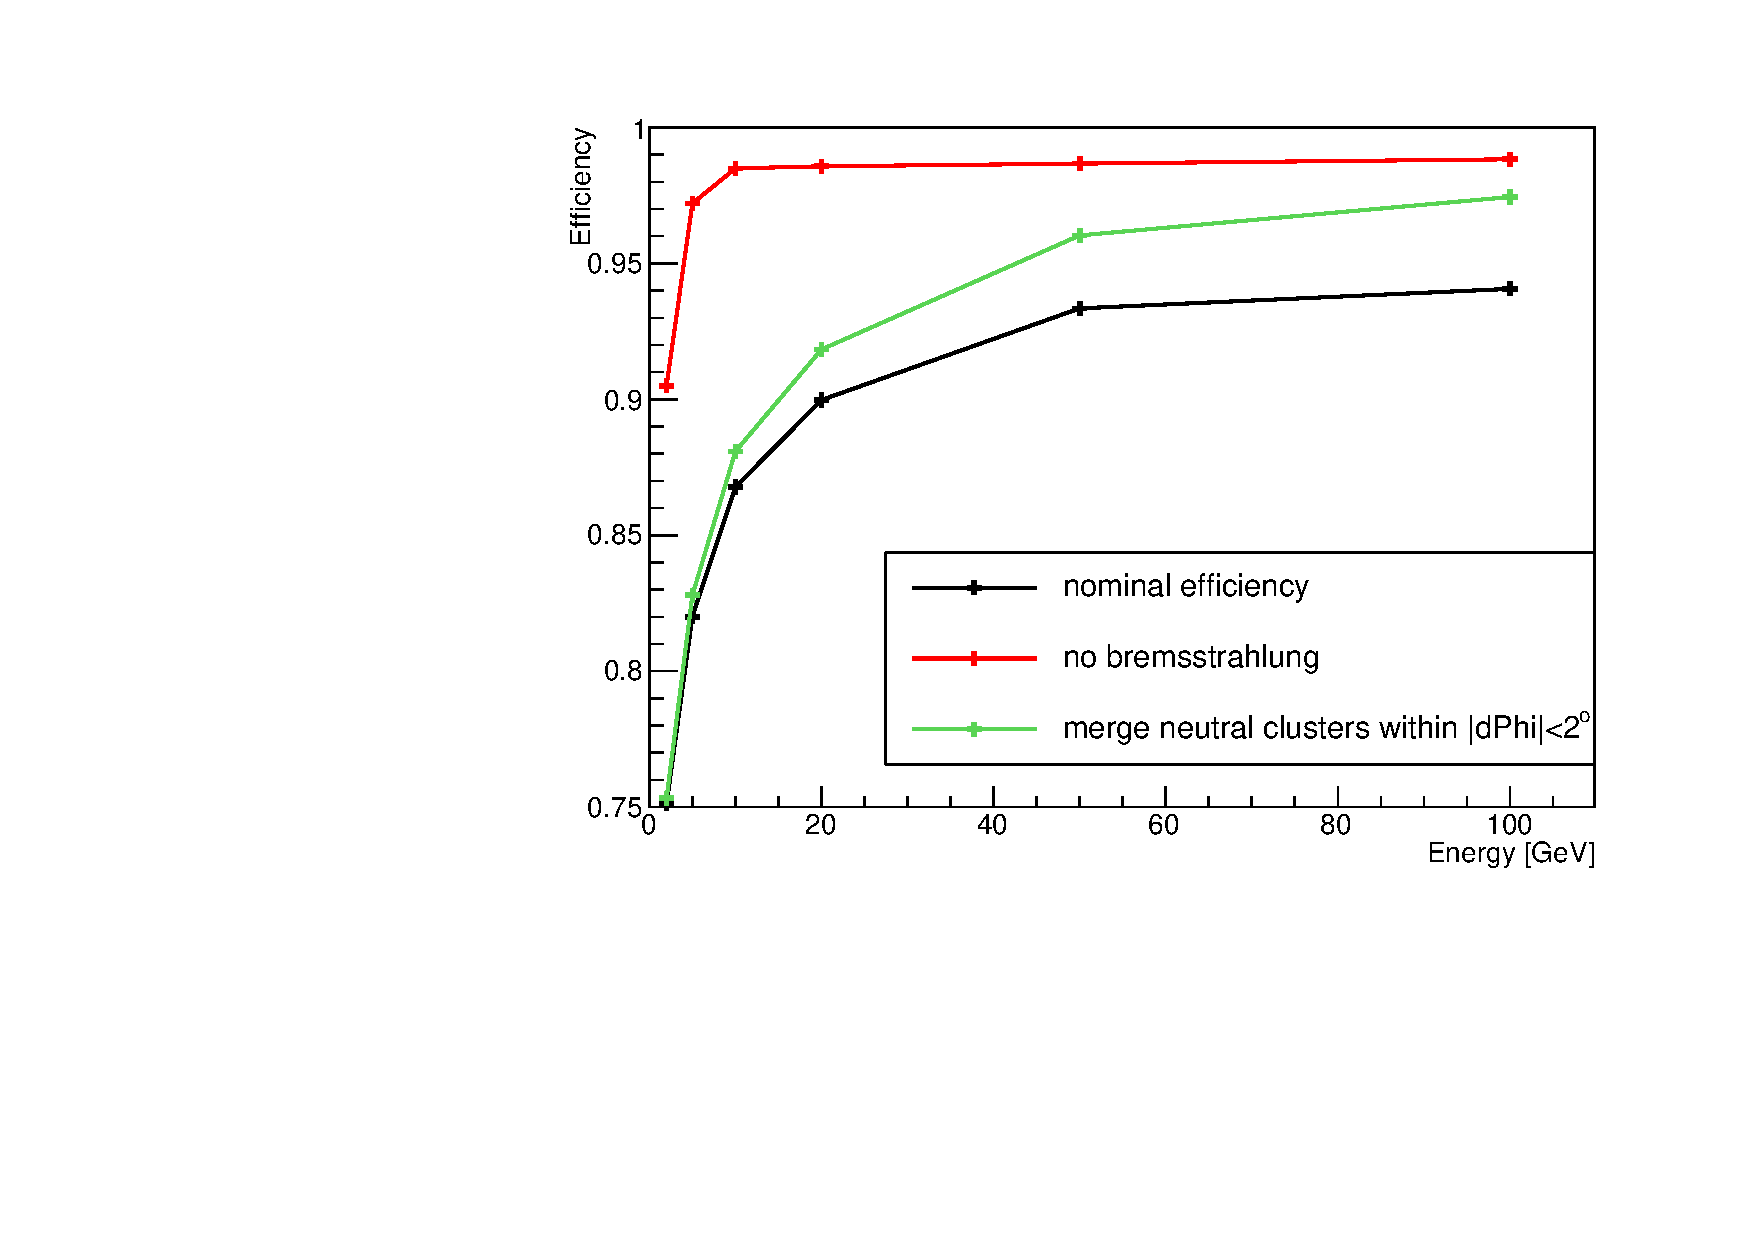
\includegraphics[width=9cm]{/home/oviazlo/Desktop/beamerPresentations/FCCee/pictures/oct11_2017/test.pdf}};
\node [Box] at (\xRefPosOne-1.2,\yRefPosOne+3.9) (box){%
\myCenterBox{FCCee}
}; 
  
  
 \node[inner sep=0pt] (tmp) at (\xRefPosOne+4.5,\yRefPosOne+1)
  {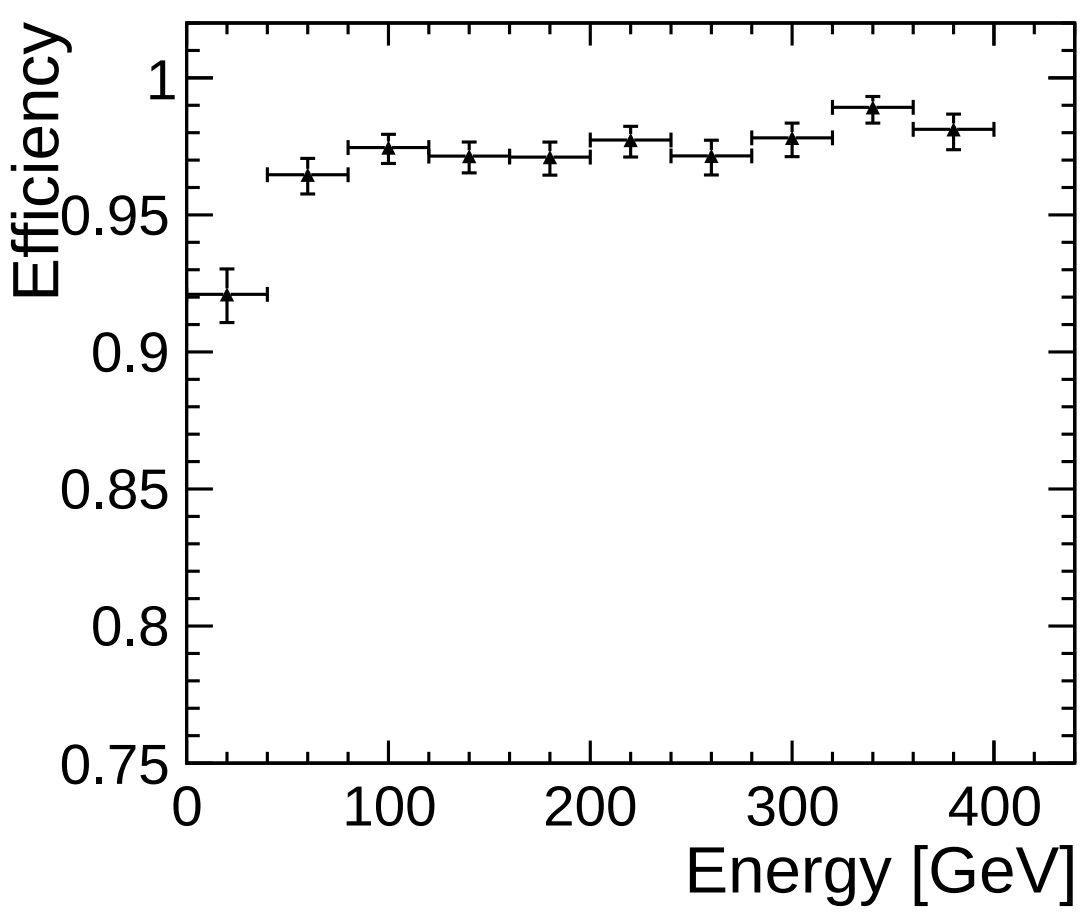
\includegraphics[width=4cm]{/home/oviazlo/Desktop/beamerPresentations/FCCee/pictures/electronEfficiency_CLIC_CDR.png}};
\node [Box] at (\xRefPosOne+4.7,\yRefPosOne+3) (box){%
\myCenterBox{CLIC CDR}
}; 
  
  \node [Box] at (\xRefPosOne,\yRefPosOne-3) (box){%
  \begin{minipage}{\textwidth}
    \begin{itemize}
      \item Merging photon clusters recover efficiency for high momentum electrons
      \item CLIC results were obtained for electron with E$>$7.5 GeV (and angle matching)

    \end{itemize}
  \end{minipage}
};
  
\end{tikzpicture}
\end{frame}
%*****************************************************************************

%*****************************************************************************
\begin{frame}{\large \large Electron $\Delta$Phi (signal PFO, second energetic PFO)}
\renewcommand{\yRefPosOne}{1.5}
\renewcommand{\xRefPosOne}{1.5}
\renewcommand{\xRefIncrementOne}{7.5}
\begin{tikzpicture}[overlay]

  \node[inner sep=0pt] (tmp) at (\xRefPosOne,\yRefPosOne)
  {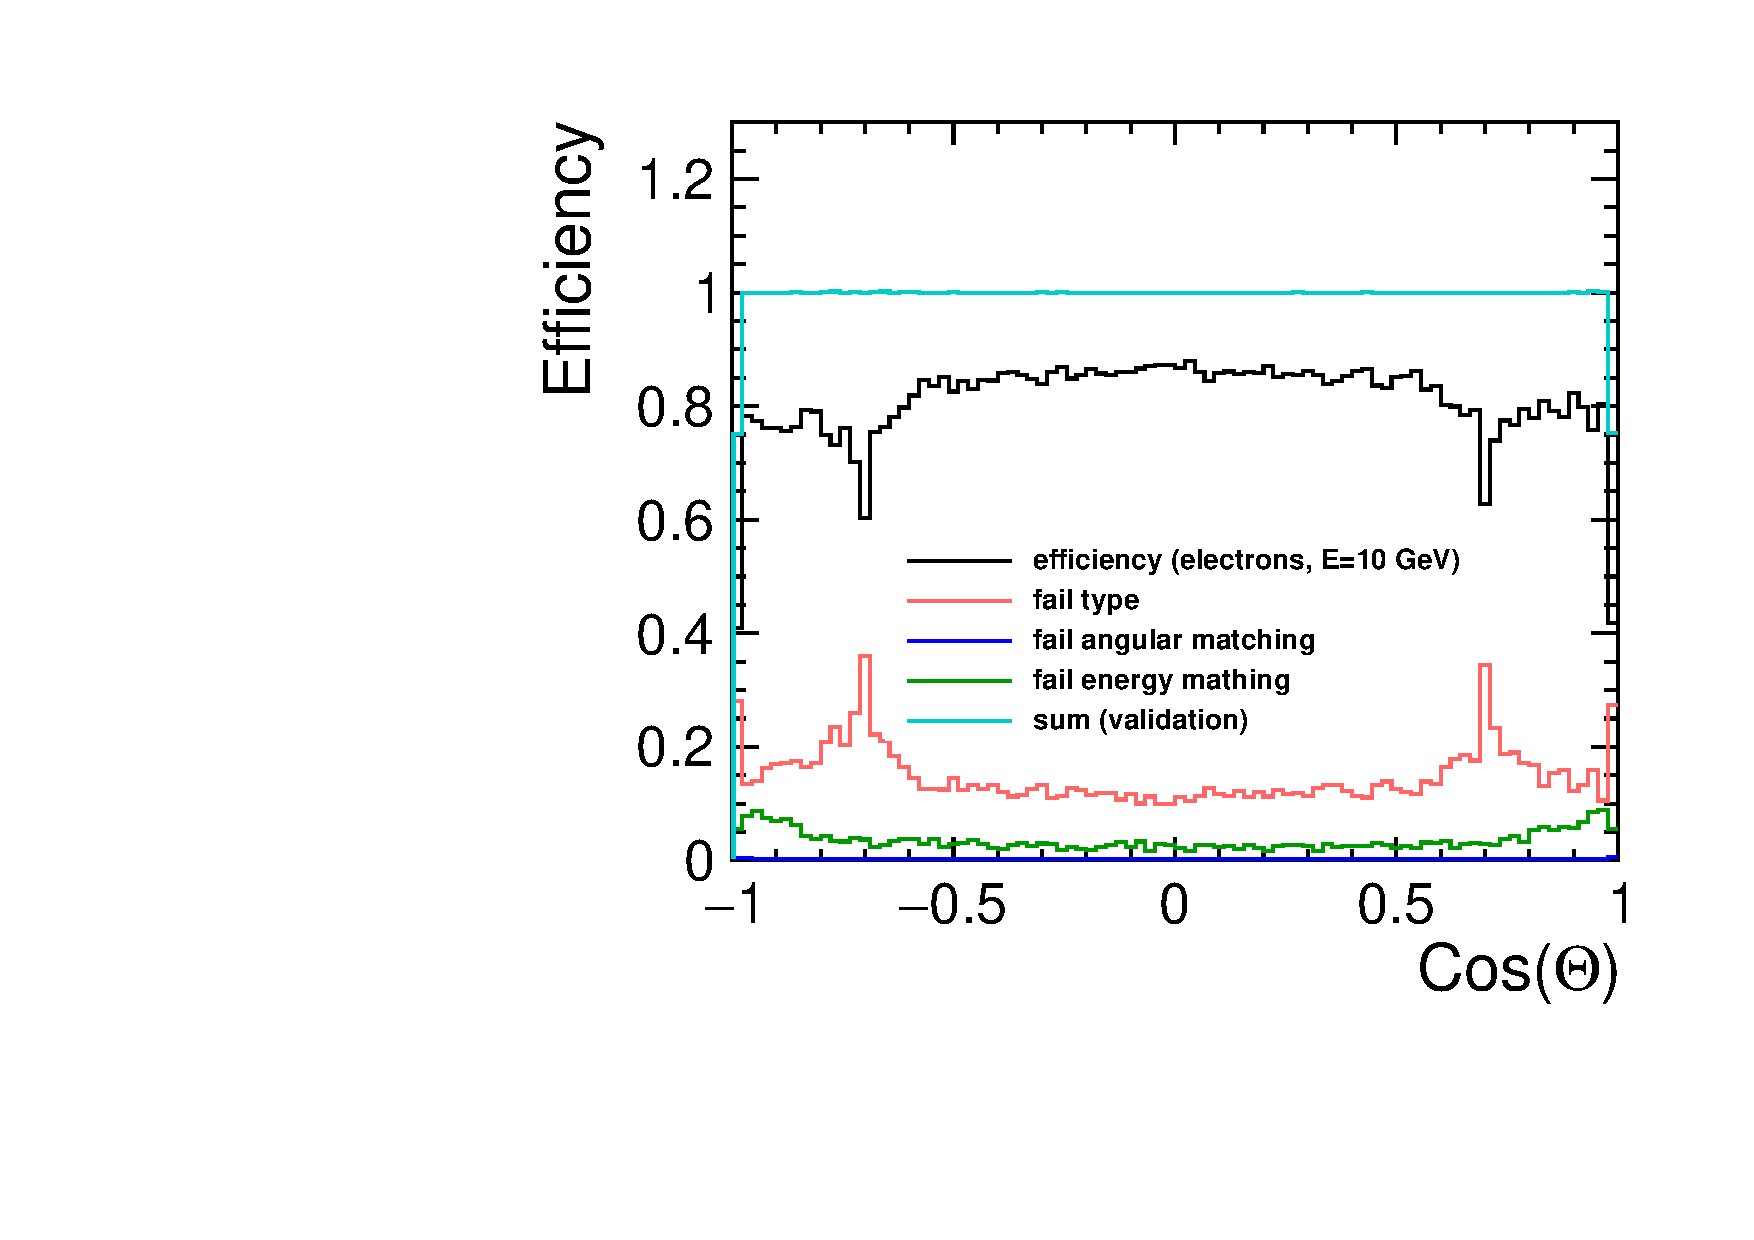
\includegraphics[width=4cm]{/home/oviazlo/Desktop/beamerPresentations/FCCee/pictures/oct11_2017/pg_0001.pdf}};

  \node[inner sep=0pt] (tmp) at (\xRefPosOne+4,\yRefPosOne)
  {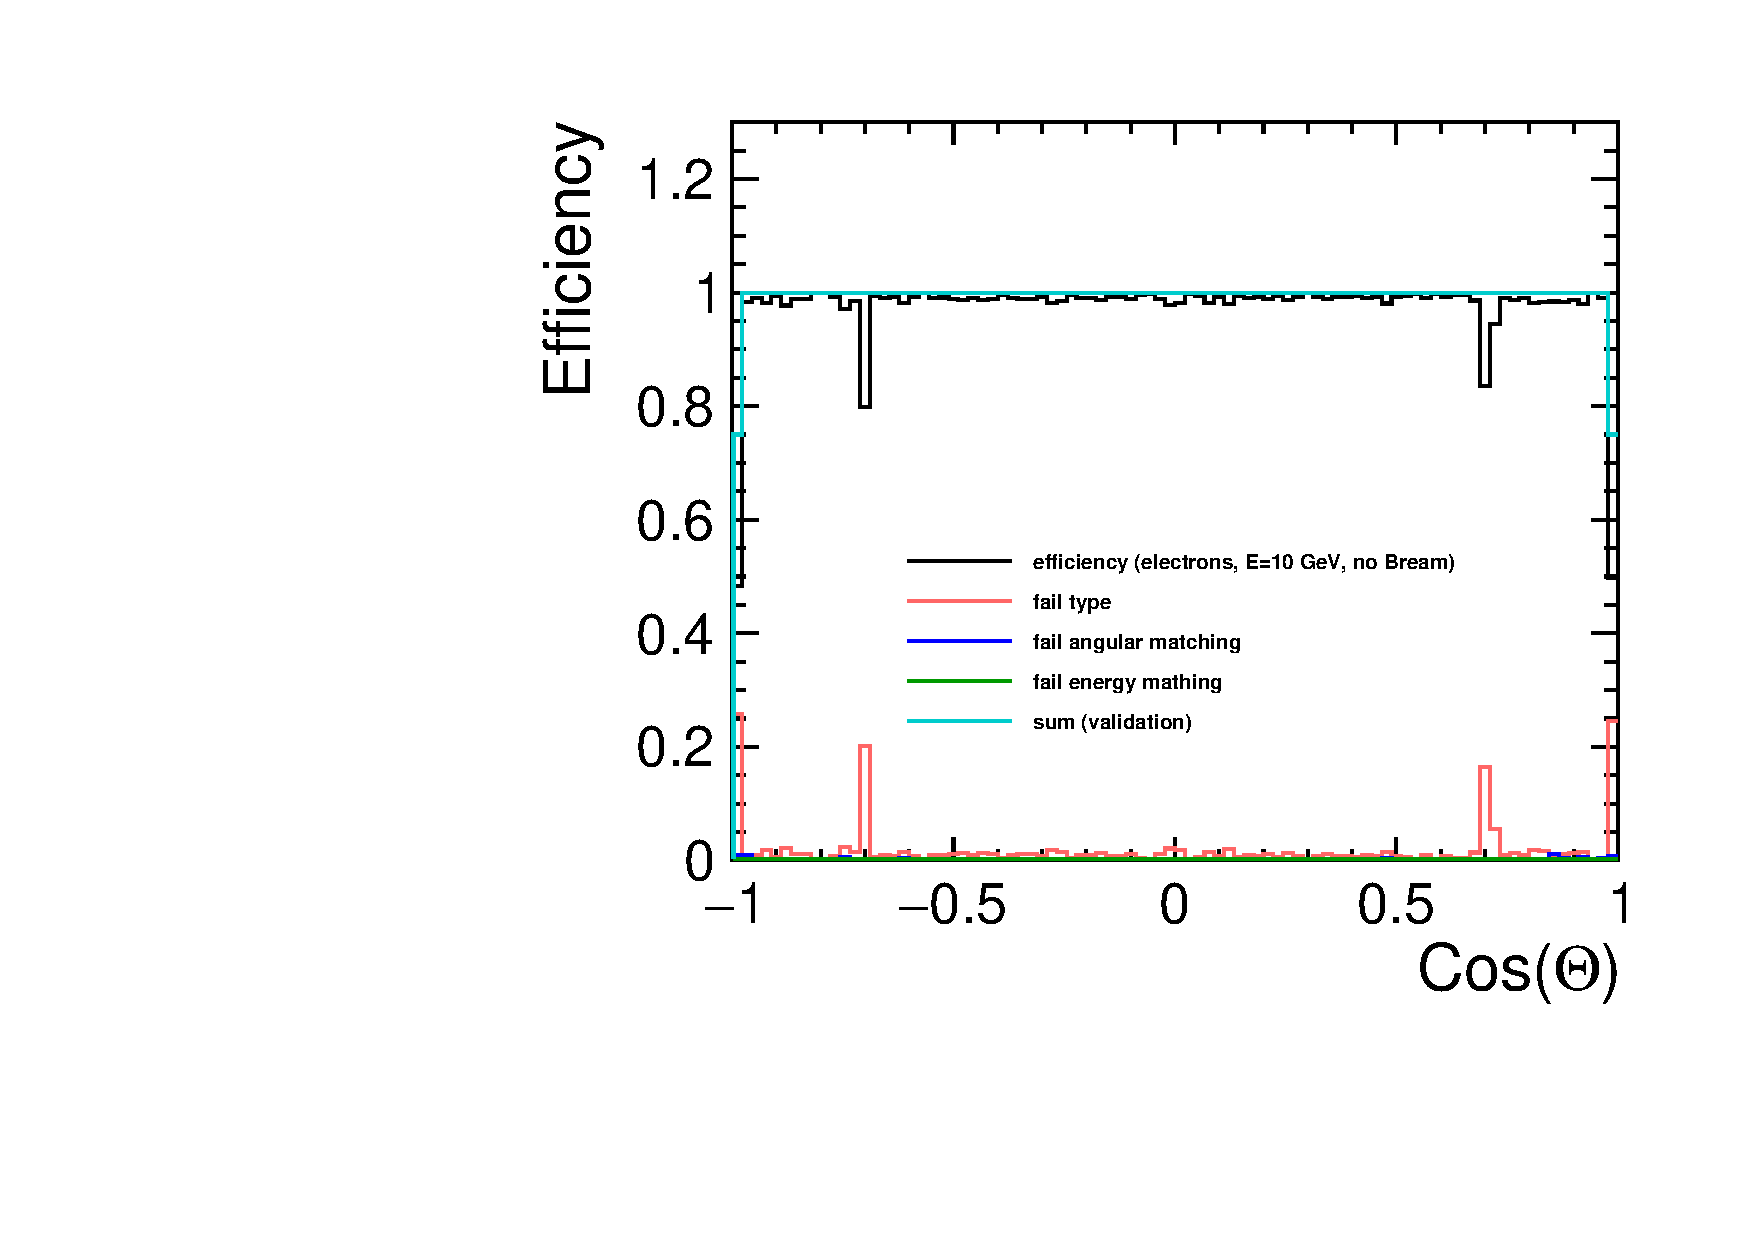
\includegraphics[width=4cm]{/home/oviazlo/Desktop/beamerPresentations/FCCee/pictures/oct11_2017/pg_0002.pdf}};
  
  \node[inner sep=0pt] (tmp) at (\xRefPosOne+8,\yRefPosOne)
  {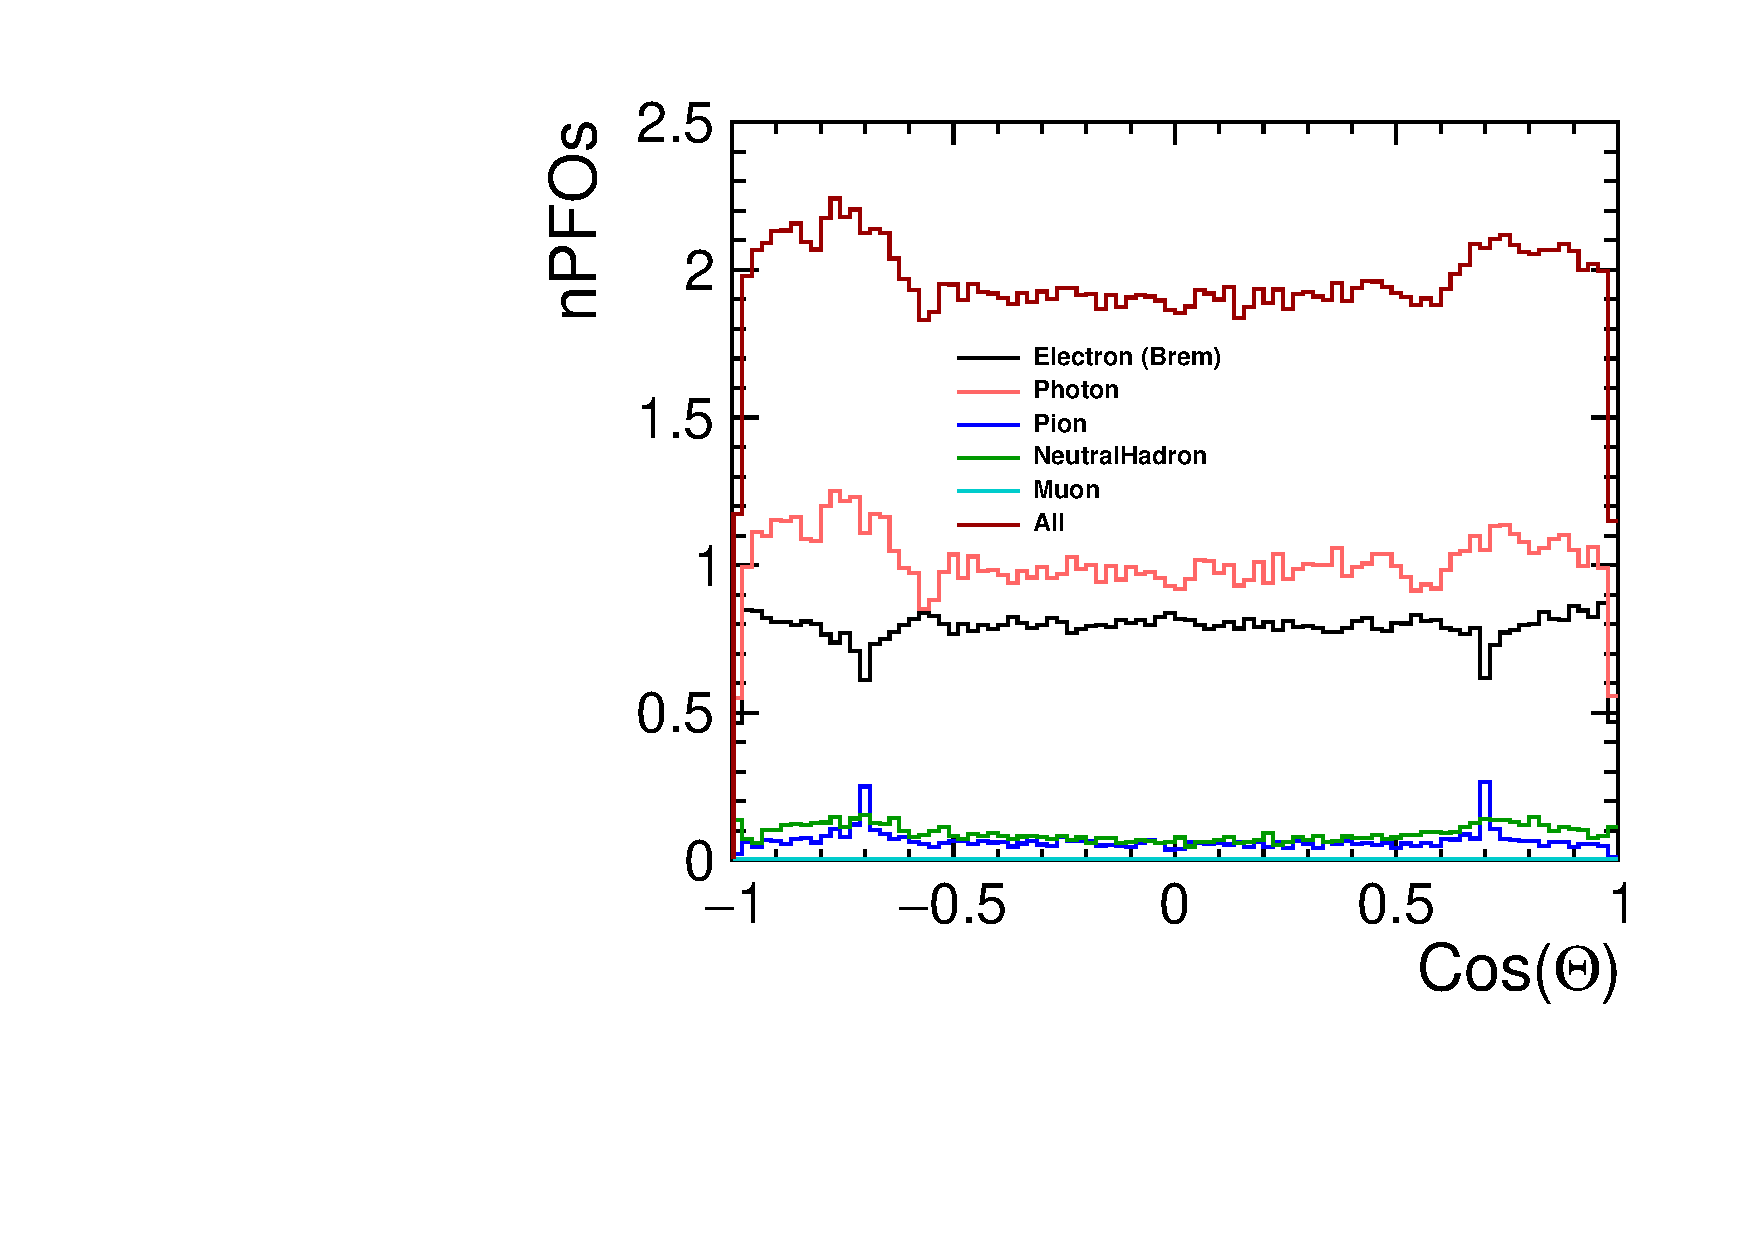
\includegraphics[width=4cm]{/home/oviazlo/Desktop/beamerPresentations/FCCee/pictures/oct11_2017/pg_0003.pdf}};
  
  \node[inner sep=0pt] (tmp) at (\xRefPosOne,\yRefPosOne-3.5)
  {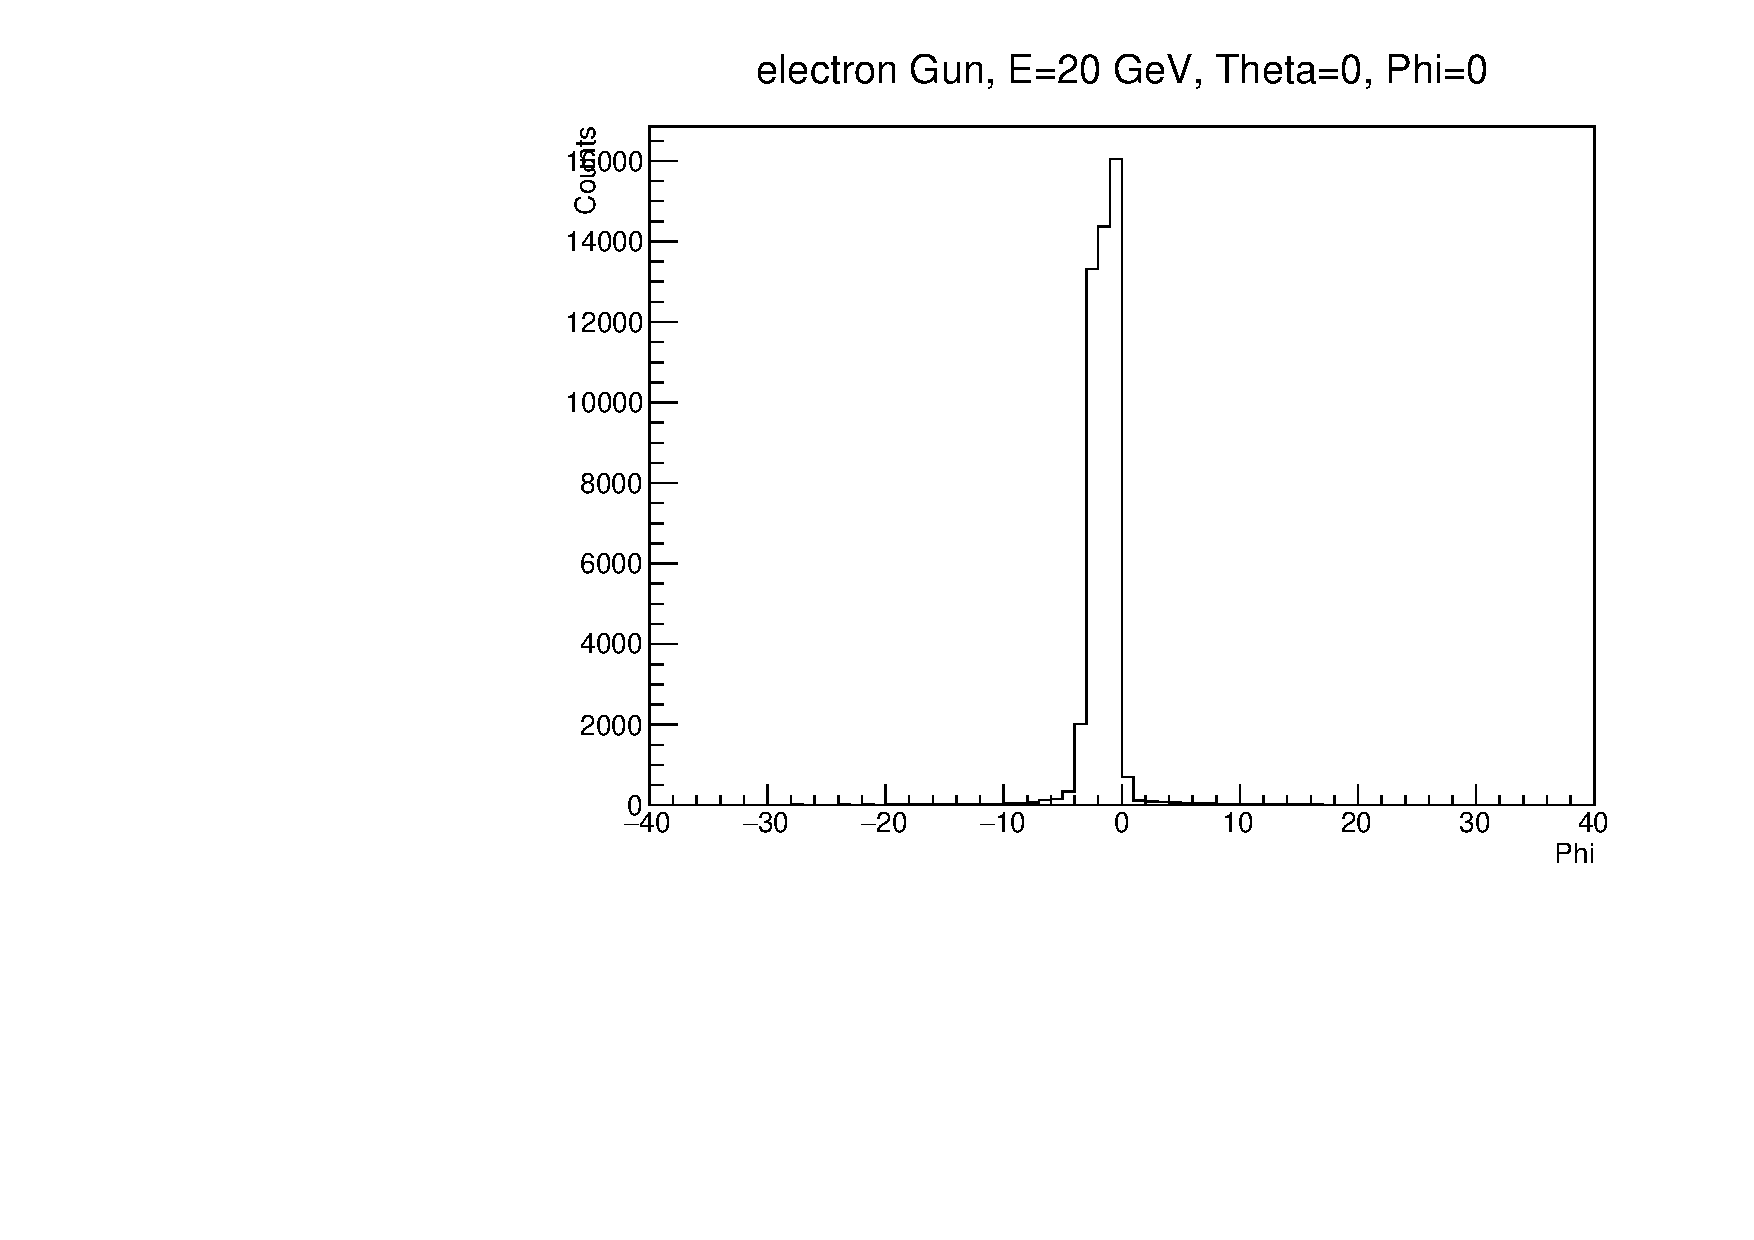
\includegraphics[width=4cm]{/home/oviazlo/Desktop/beamerPresentations/FCCee/pictures/oct11_2017/pg_0004.pdf}};
  
  \node[inner sep=0pt] (tmp) at (\xRefPosOne+4,\yRefPosOne-3.5)
  {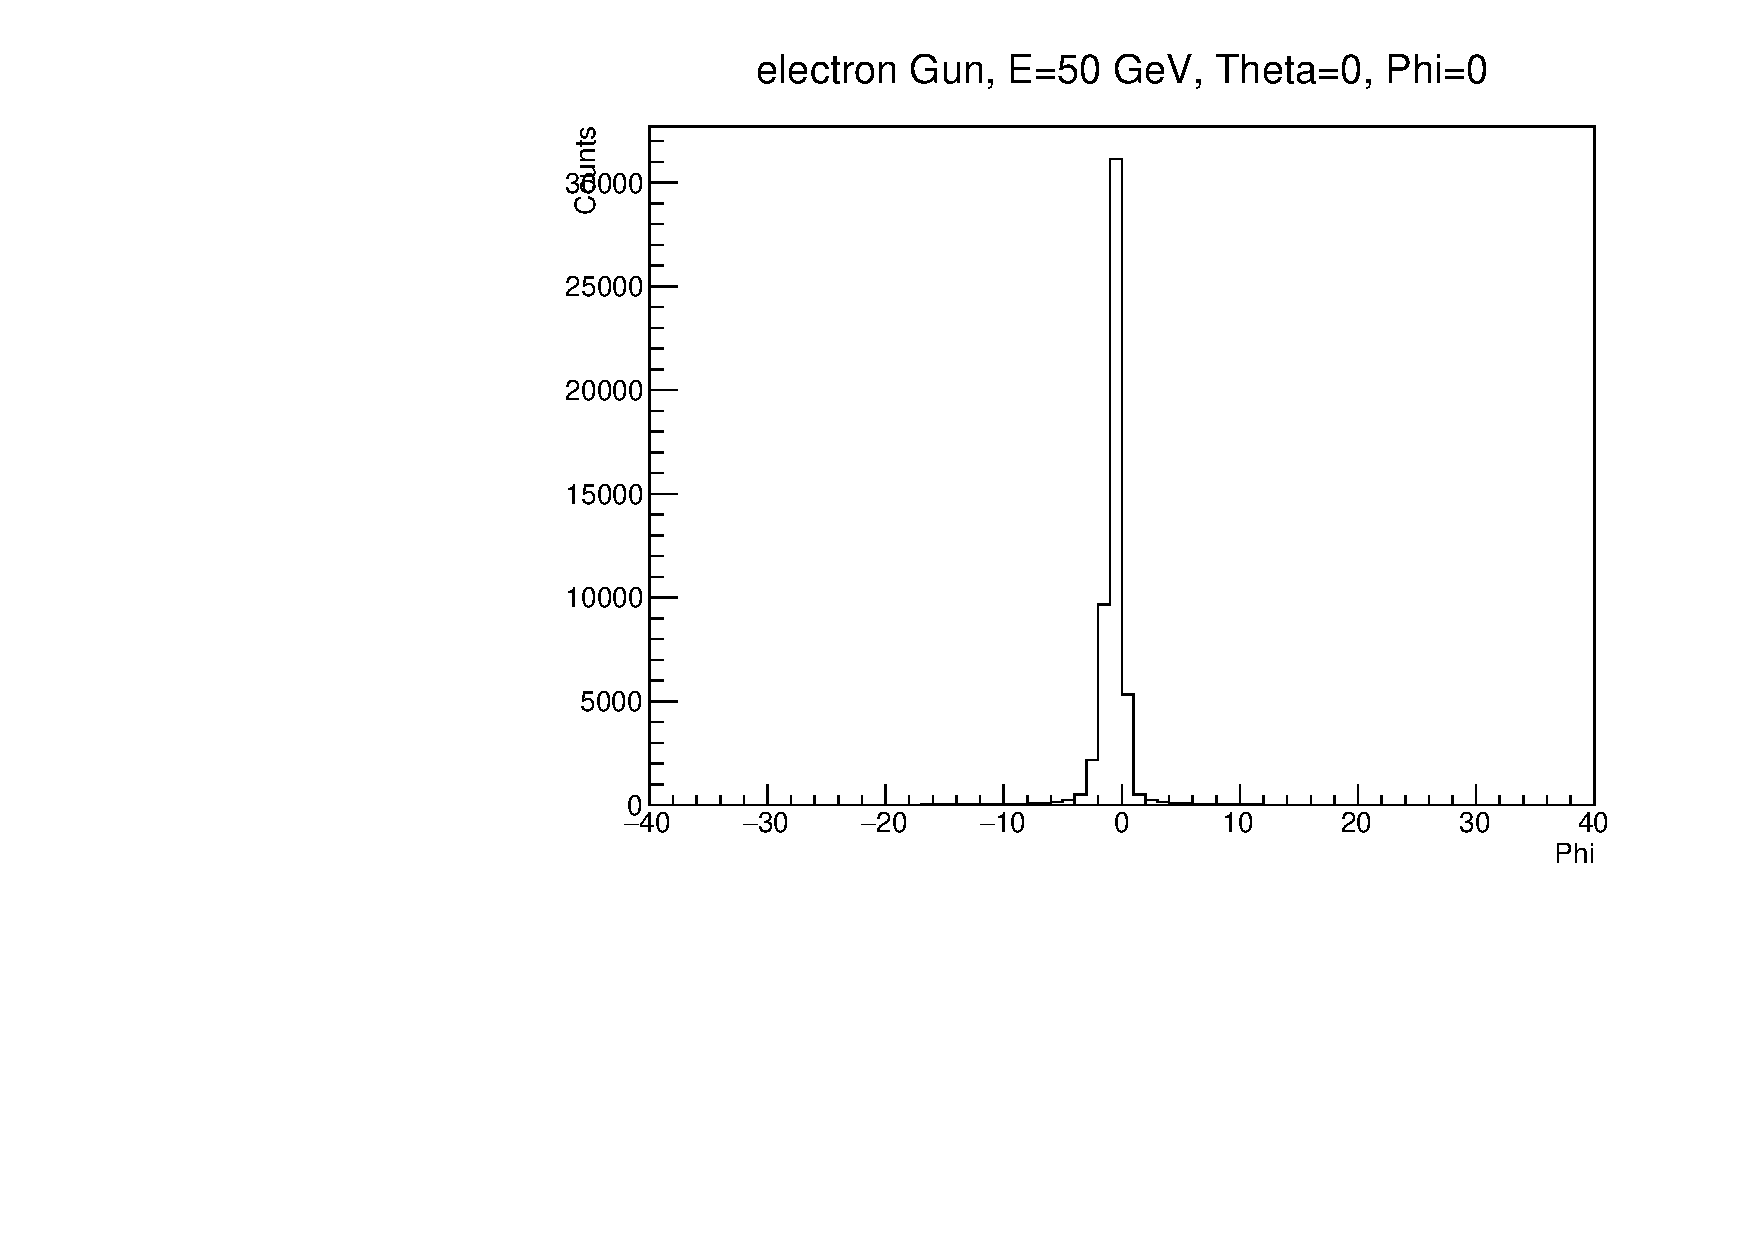
\includegraphics[width=4cm]{/home/oviazlo/Desktop/beamerPresentations/FCCee/pictures/oct11_2017/pg_0005.pdf}};
  
  \node[inner sep=0pt] (tmp) at (\xRefPosOne+8,\yRefPosOne-3.5)
  {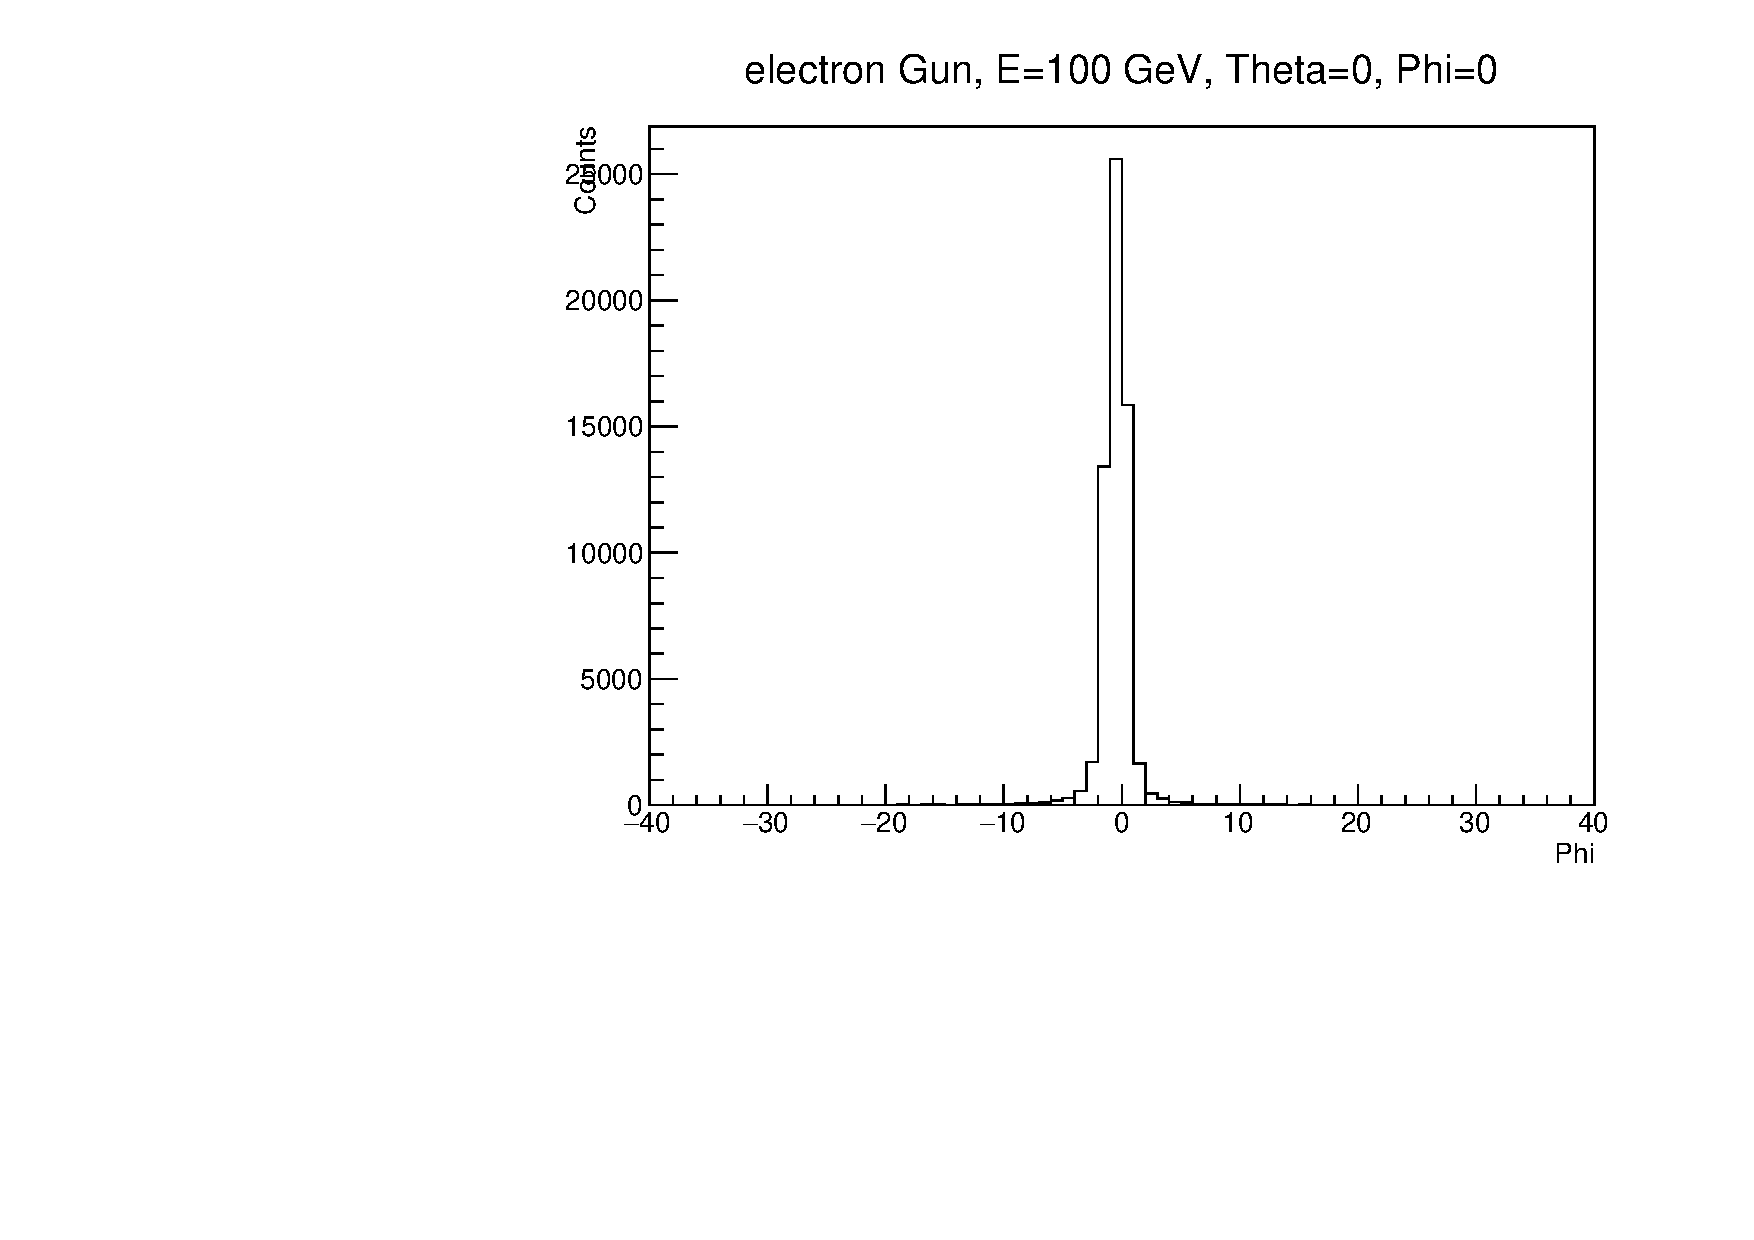
\includegraphics[width=4cm]{/home/oviazlo/Desktop/beamerPresentations/FCCee/pictures/oct11_2017/pg_0006.pdf}};
  
  \node [Box] at (\xRefPosOne+4,\yRefPosOne-5.5) (box){%
    \begin{minipage}{\textwidth}
      \begin{itemize}
	\item Bremsstrahlung from high-momentum electrons are more collimated around electron than for curved low-momentum tracks
      \end{itemize}
    \end{minipage}
  };
  
\end{tikzpicture}
\end{frame}
%*****************************************************************************

%*****************************************************************************
\begin{frame}{}
  \begin{tikzpicture}[overlay]
    \node[right] (textNode) at (3,0) {
      { \large \bf K$_{L}^{0}$ ID efficiency in transition region }
    };
  \end{tikzpicture}
\end{frame}
%*****************************************************************************

%*****************************************************************************
\begin{frame}{\large \large K$_{L}^{0}$ ID efficiency}
\renewcommand{\yRefPosOne}{-0.5}
\renewcommand{\xRefPosOne}{4.2}
\renewcommand{\xRefIncrementOne}{7.5}
\begin{tikzpicture}[overlay]

 \node[inner sep=0pt] (tmp) at (\xRefPosOne-1.7,\yRefPosOne+0.7)
  {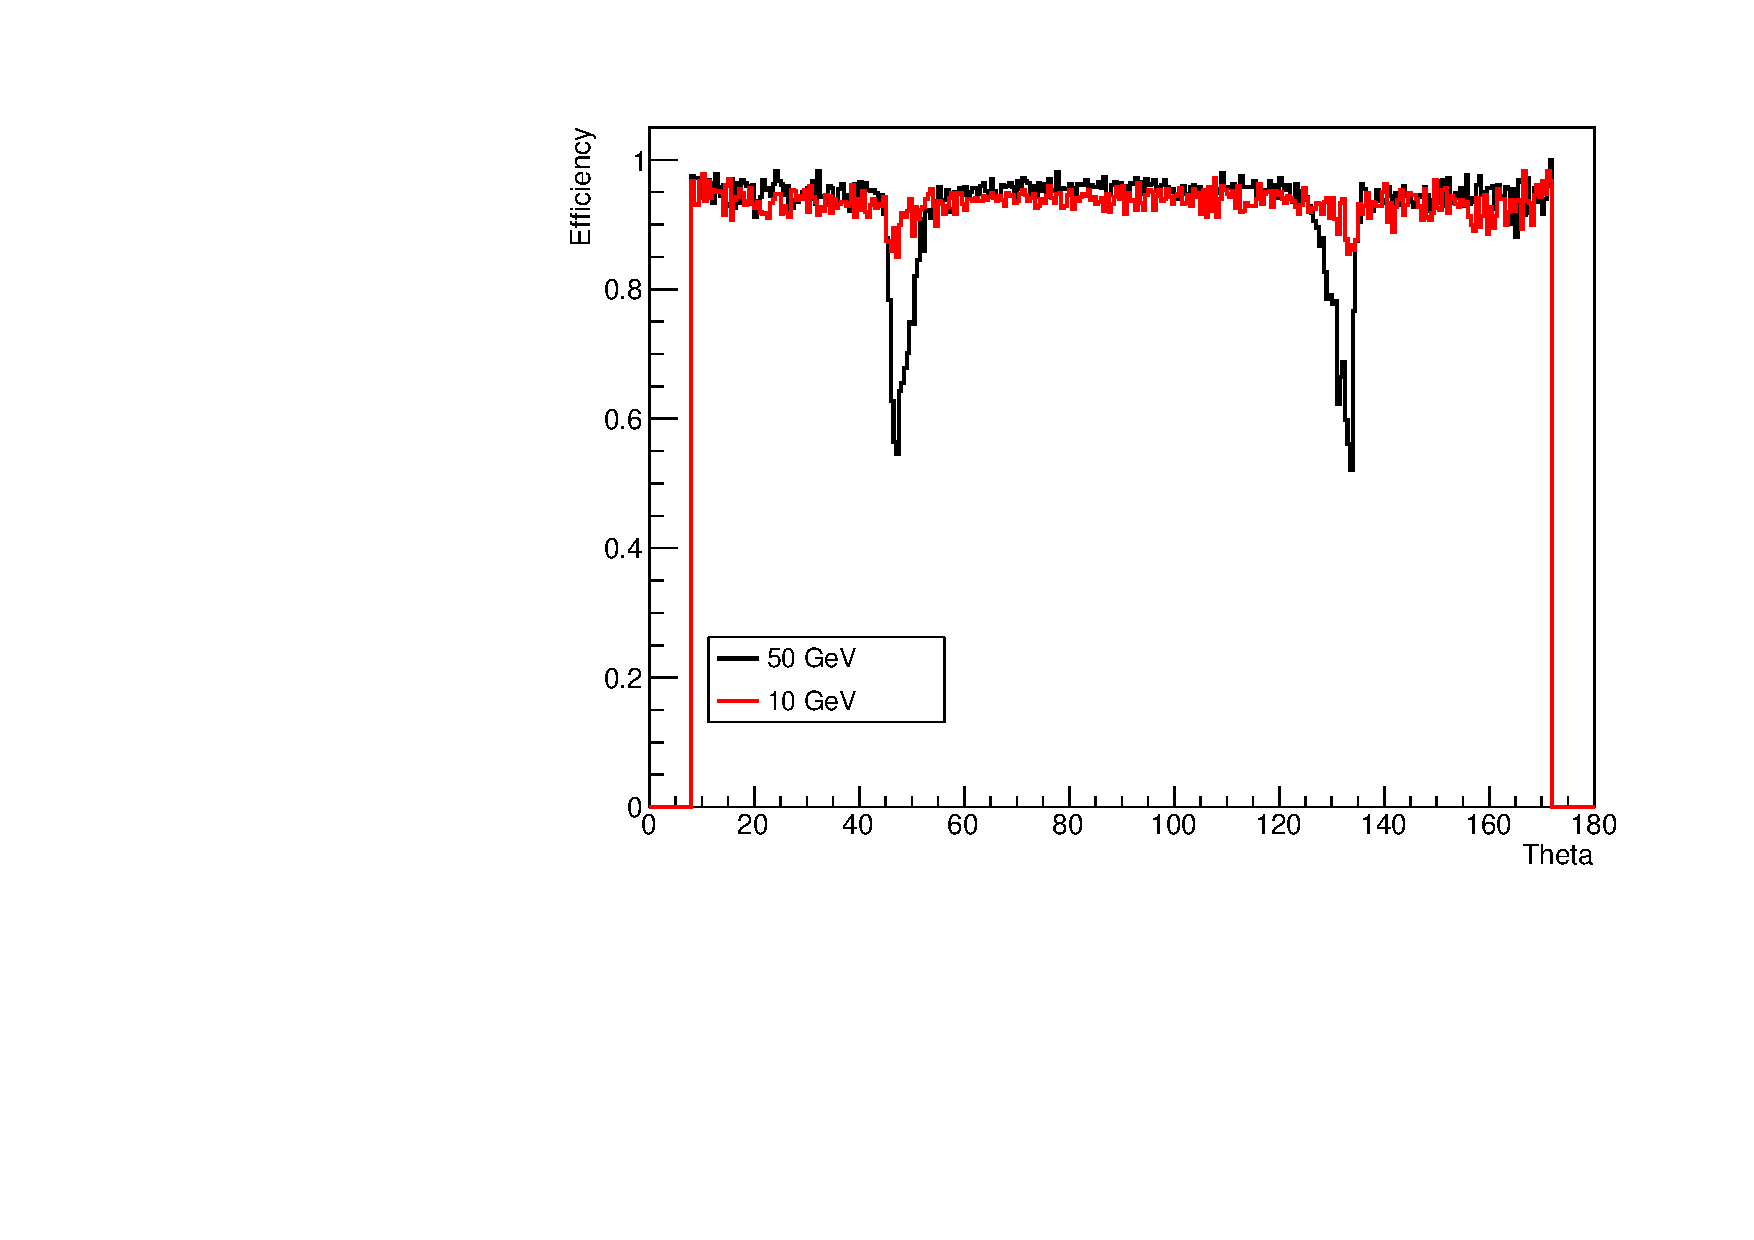
\includegraphics[width=6cm]{eff_vs_theta_10_50_GeV_comp.pdf}};
 
  
  
 \node[inner sep=0pt] (tmp) at (\xRefPosOne+4.5,\yRefPosOne+0.7)
  {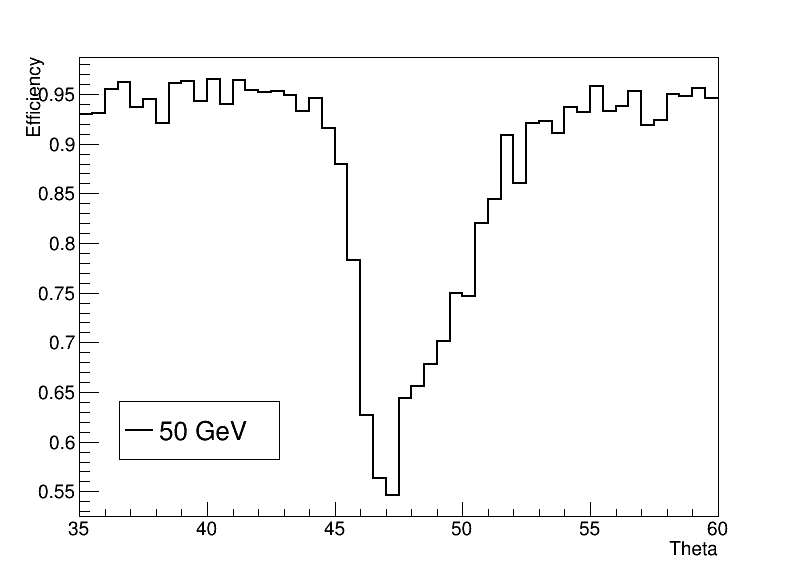
\includegraphics[width=6cm]{eff_vs_theta_50GeV_zoom.png}};

  
  \node [Box] at (\xRefPosOne+0.7,\yRefPosOne-3) (box){%
  \begin{minipage}{\textwidth}
    \begin{itemize}
      \item Efficiency drop in the region 45-52 degrees for high-energetic kaons

    \end{itemize}
  \end{minipage}
};
  
\end{tikzpicture}
\end{frame}
%*****************************************************************************

%*****************************************************************************
\begin{frame}{\large \large K$_{L}^{0}$ ID efficiency}
\renewcommand{\yRefPosOne}{-0.5}
\renewcommand{\xRefPosOne}{4.2}
\renewcommand{\xRefIncrementOne}{7.5}
\begin{tikzpicture}[overlay]

 \node[inner sep=0pt] (tmp) at (\xRefPosOne-1.4,\yRefPosOne+0.7)
  {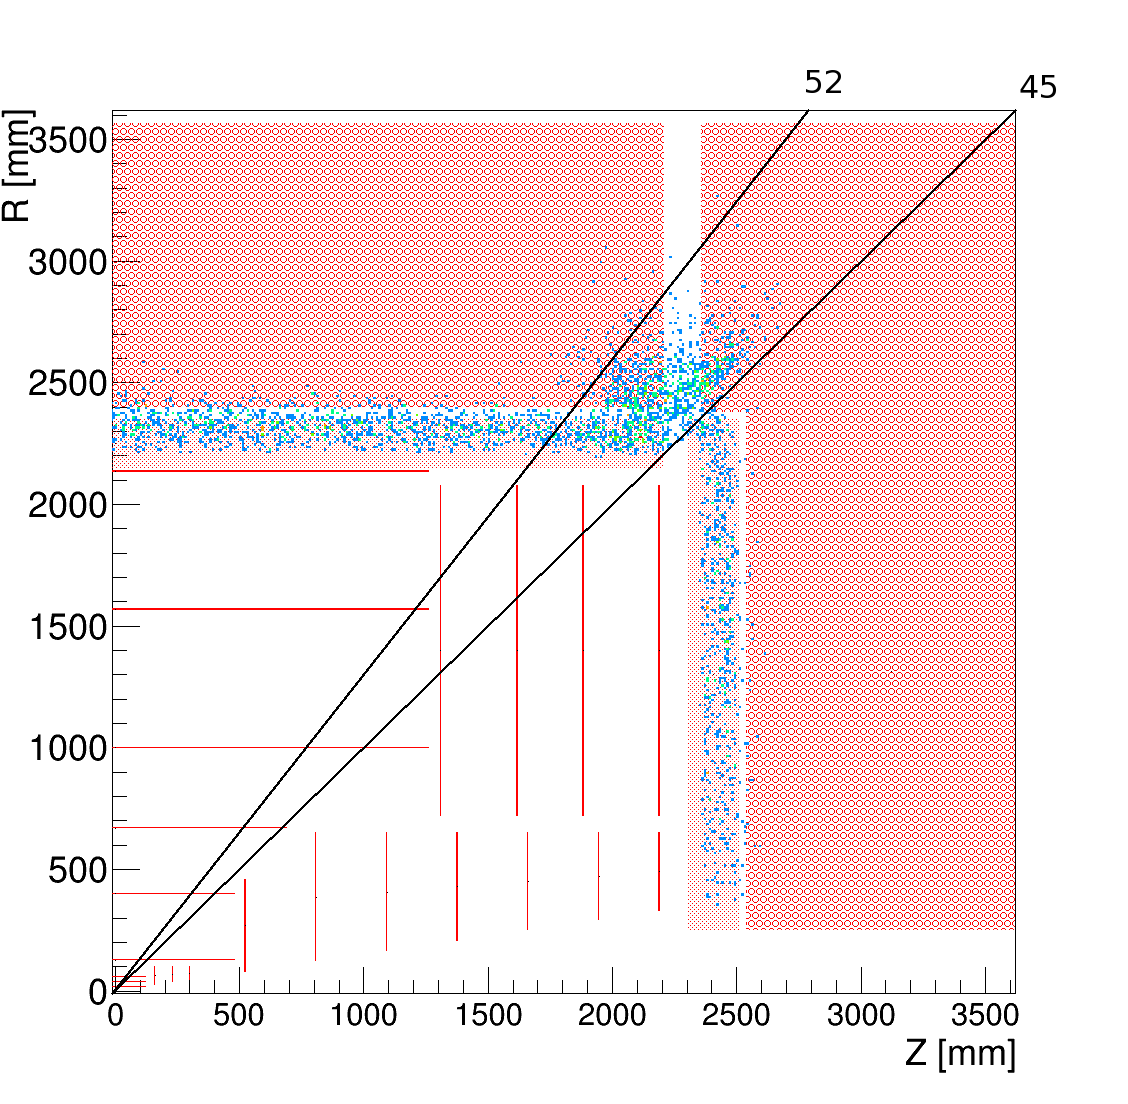
\includegraphics[width=7cm]{kaon0L_50GeV_fakes.png}};
 
  
  
 \node[inner sep=0pt] (tmp) at (\xRefPosOne+4.5,\yRefPosOne+0.7)
  {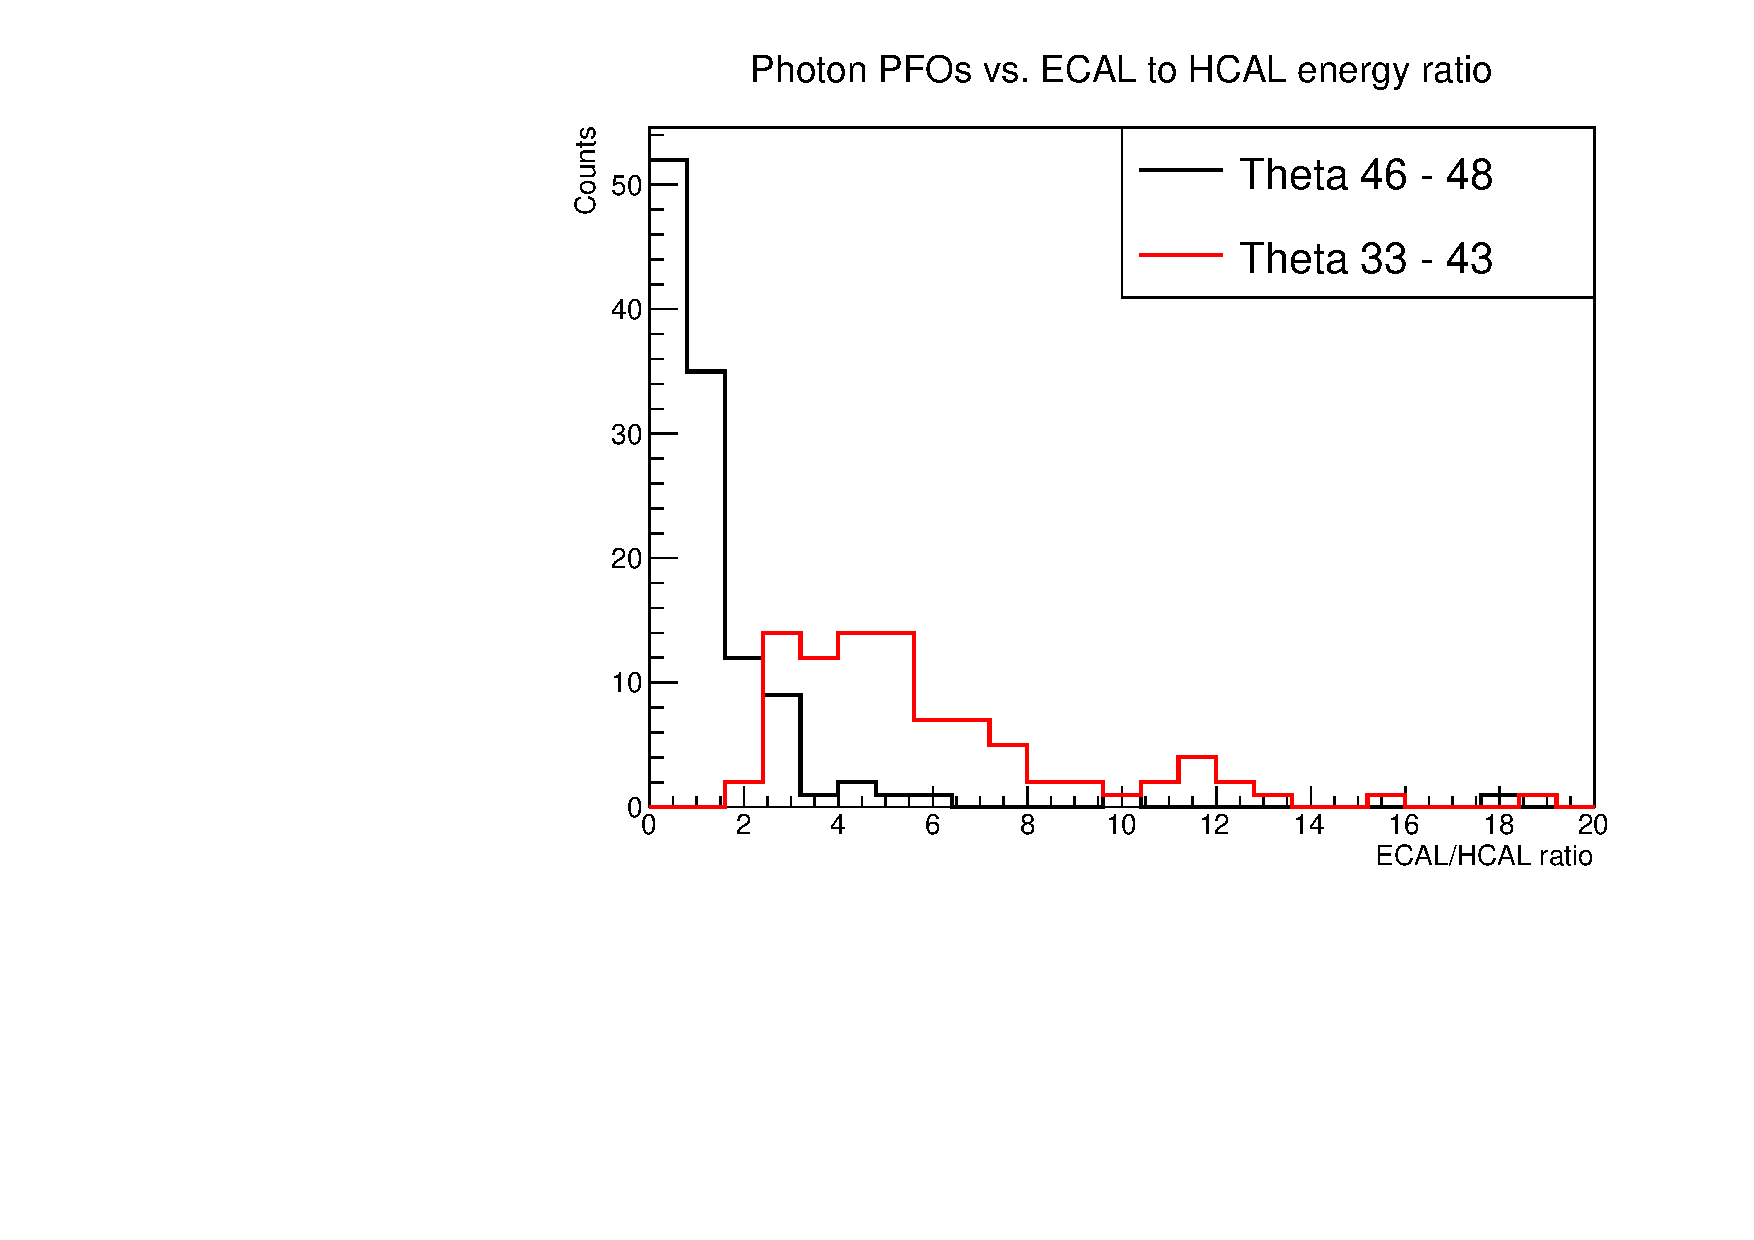
\includegraphics[width=5.5cm]{ecal_to_hcal_ratio_photonPFO.pdf}};

  
  \node [Box] at (\xRefPosOne+0.7,\yRefPosOne-3.3) (box){%
  \begin{minipage}{\textwidth}
    \begin{itemize}
      \item Inefficiency is caused by misidentification of neutral clusters as photons
      \item ECAL/HCAL energy ratio of misreconstructed clusters in the transition has different profile than ``fakes'' in non-transition region

    \end{itemize}
  \end{minipage}
};
  
\end{tikzpicture}
\end{frame}
%*****************************************************************************

%*****************************************************************************
\begin{frame}{\large \large K$_{L}^{0}$ energy reconstruction}
\renewcommand{\yRefPosOne}{-0.5}
\renewcommand{\xRefPosOne}{4.2}
\renewcommand{\xRefIncrementOne}{7.5}
\begin{tikzpicture}[overlay]

 \node[inner sep=0pt] (tmp) at (\xRefPosOne-1.4,\yRefPosOne+0.7)
  {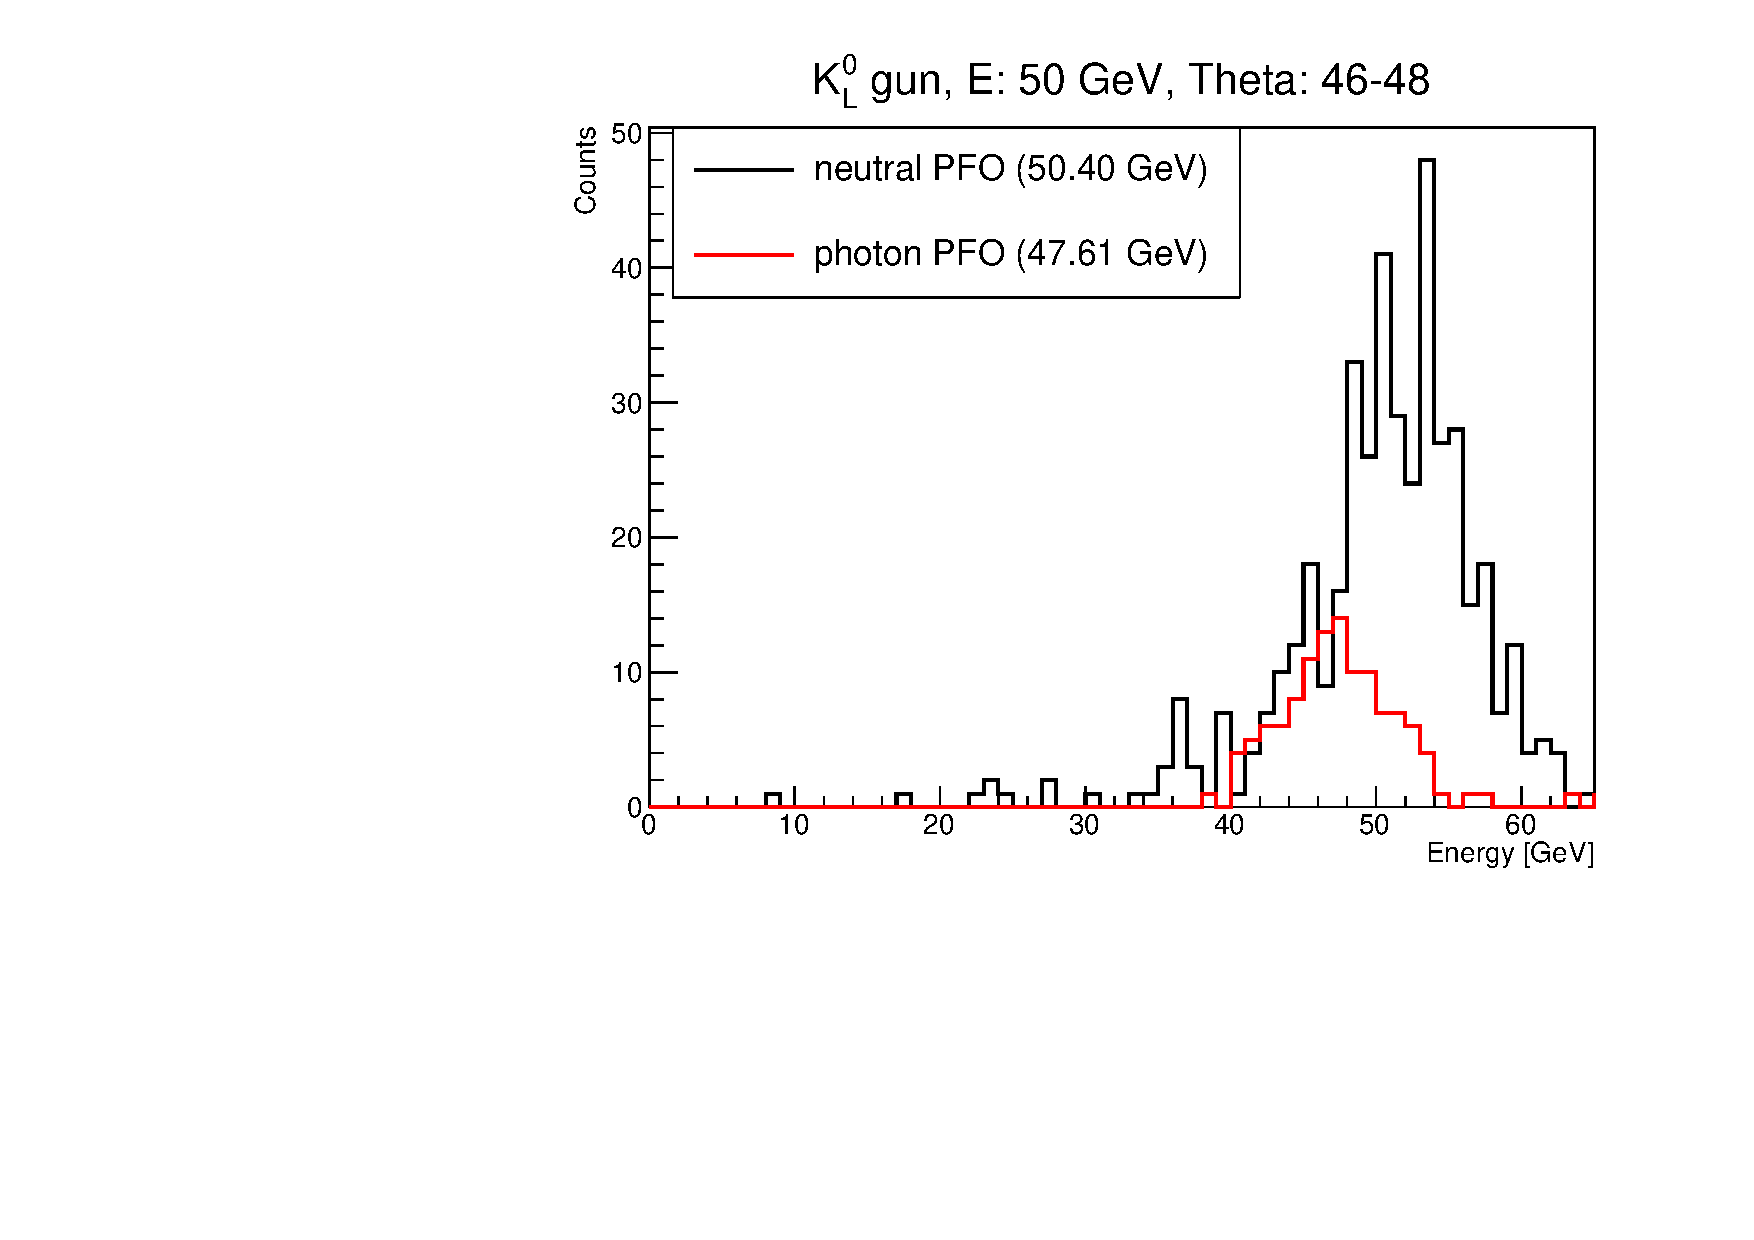
\includegraphics[width=6cm]{crack_energy.pdf}};
 
  
  
 \node[inner sep=0pt] (tmp) at (\xRefPosOne+4.5,\yRefPosOne+0.7)
  {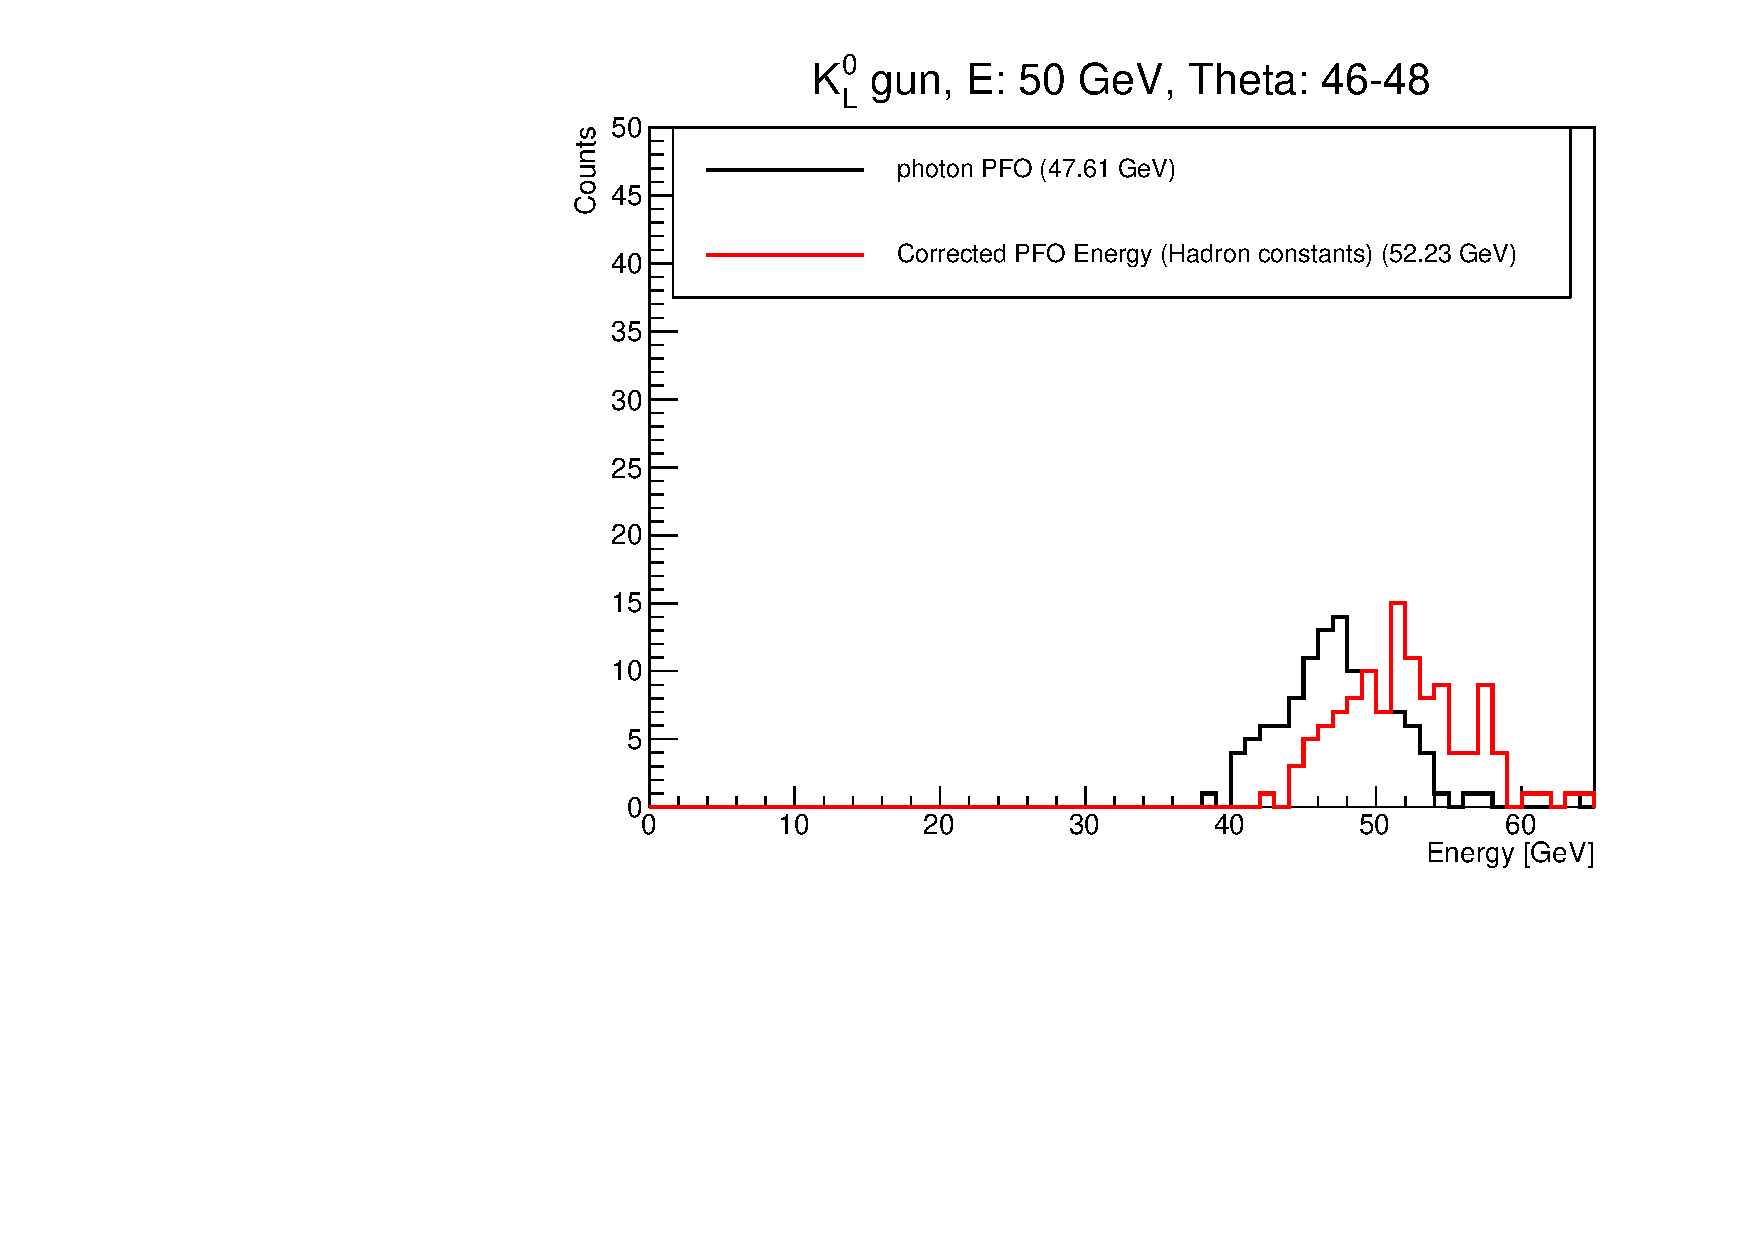
\includegraphics[width=6cm]{energy_corrections_forPhotons.pdf}};

  
  \node [Box] at (\xRefPosOne+0.7,\yRefPosOne-3) (box){%
  \begin{minipage}{\textwidth}
    \begin{itemize}
      \item For photon and neutral PFOs reconstruction different calibration constants are used:
      \begin{itemize}
       \item ECalToEM = HCalToEM = 1.024
       \item ECalToHad = 1.119; HCalToHad = 1.180
      \end{itemize}
      \item Applying hadron constants provide overestimation of the energy:
      \begin{itemize}
       \item 47.6 GeV $\to$ 52.2 GeV
      \end{itemize}
      
    \end{itemize}
  \end{minipage}
};
  
\end{tikzpicture}
\end{frame}
%*****************************************************************************


%*****************************************************************************
\begin{frame}{\large \large Examples of photon and neutral clusters}
\renewcommand{\yRefPosOne}{-0.7}
\renewcommand{\xRefPosOne}{4.2}
\renewcommand{\xRefIncrementOne}{7.5}
\begin{tikzpicture}[overlay]

 \node[inner sep=0pt] (tmp) at (\xRefPosOne-1.4,\yRefPosOne+2)
  {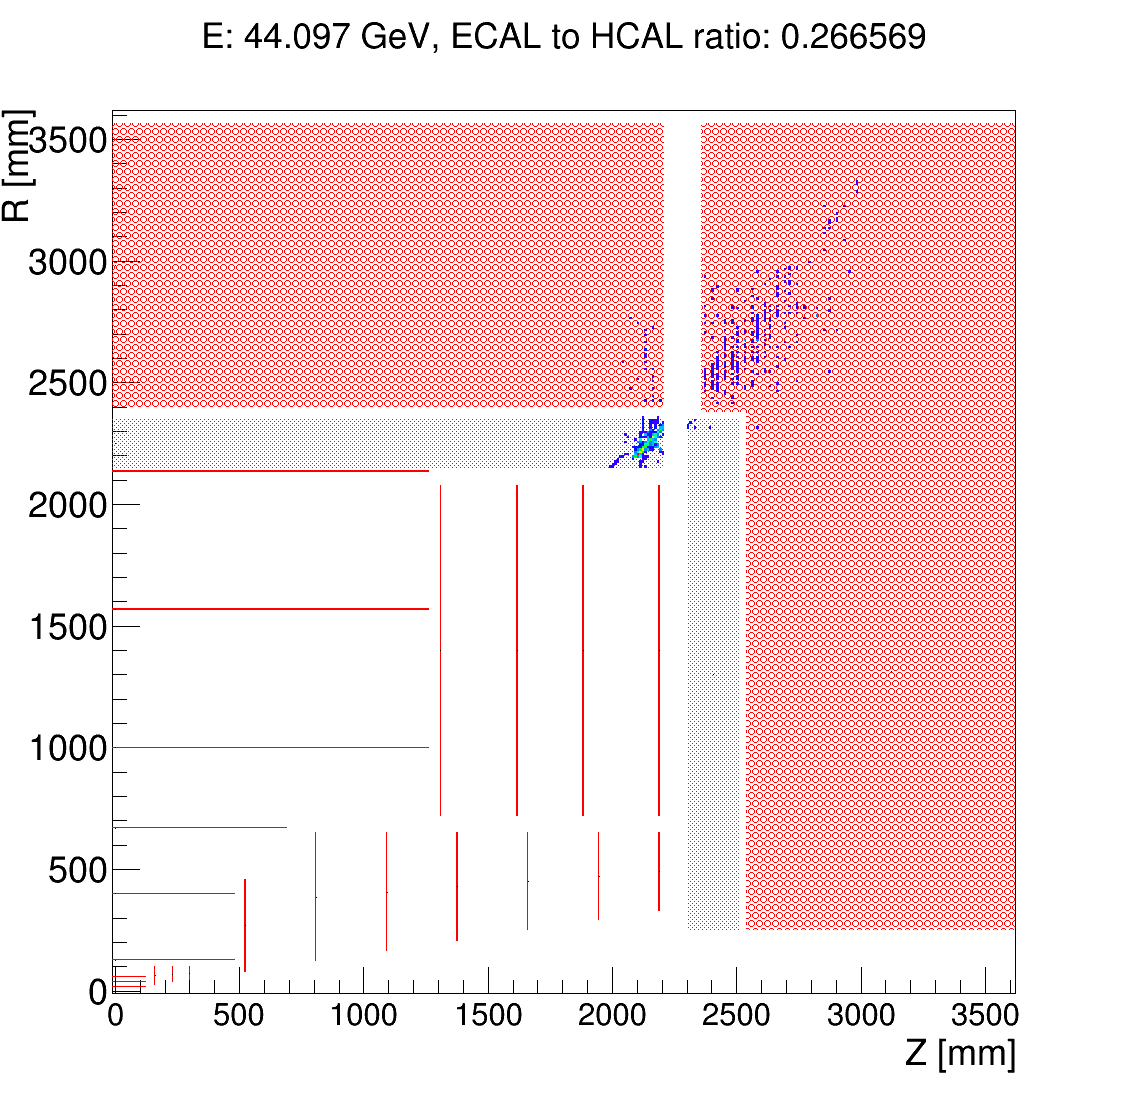
\includegraphics[width=5cm]{ex1.png}};
 
   
 \node[inner sep=0pt] (tmp) at (\xRefPosOne+4.5,\yRefPosOne+2)
  {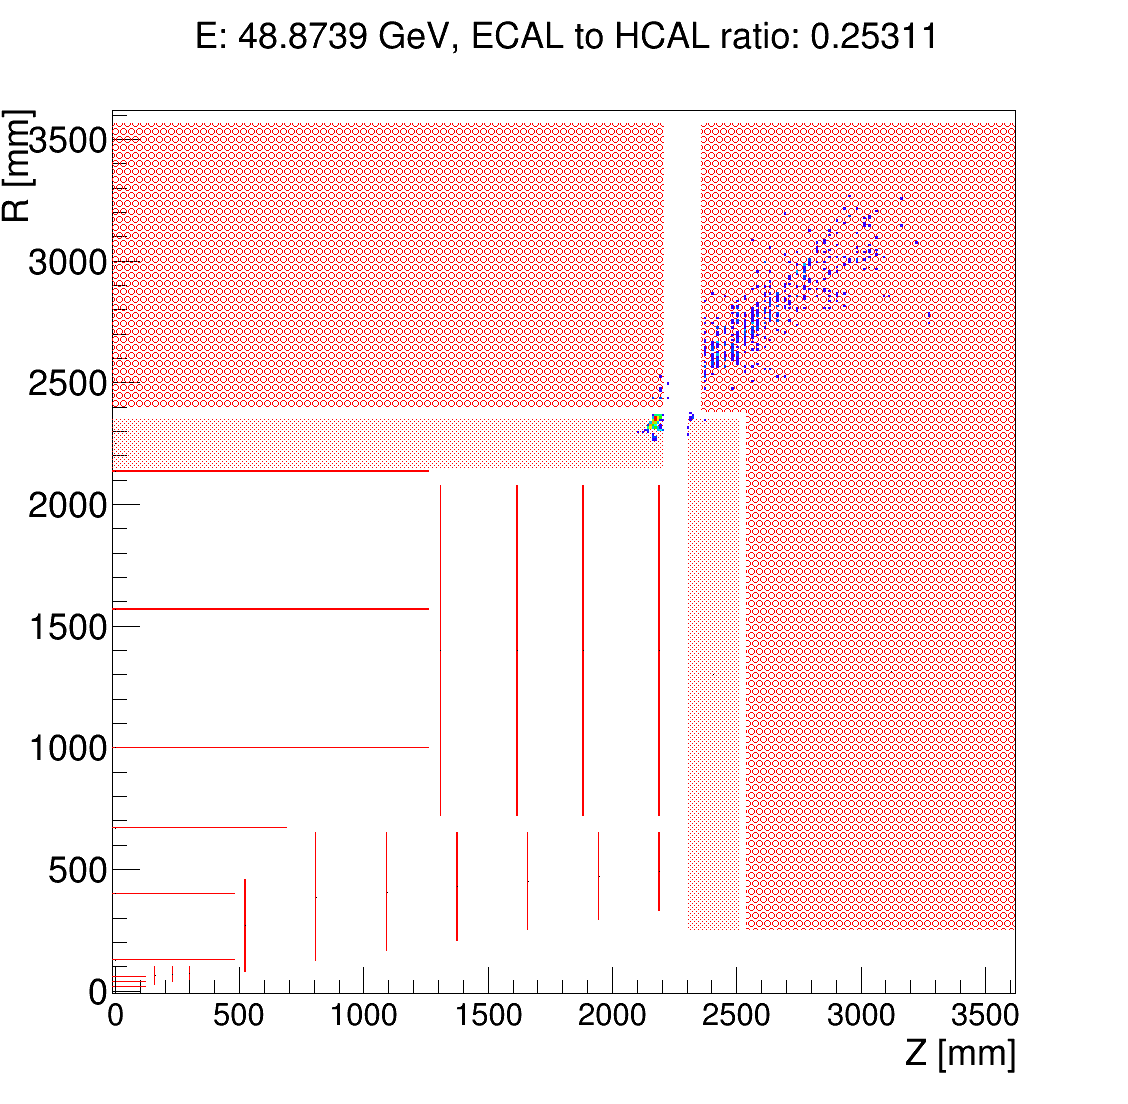
\includegraphics[width=5cm]{exHad1.png}};


    
  

 \node[inner sep=0pt] (tmp) at (\xRefPosOne-1.4,\yRefPosOne-2)
  {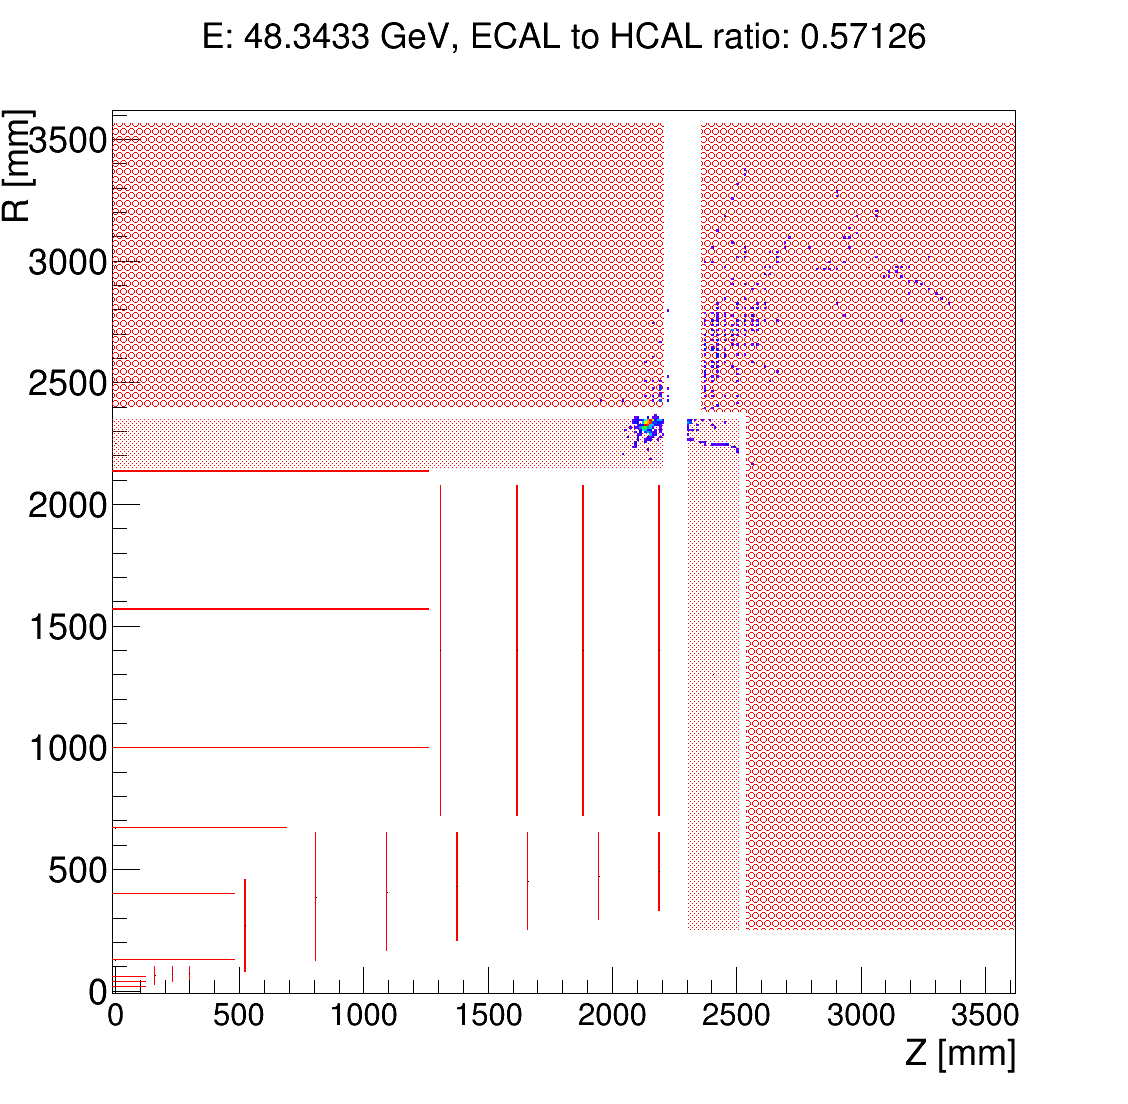
\includegraphics[width=5cm]{ex2.png}};
  
  
 \node[inner sep=0pt] (tmp) at (\xRefPosOne+4.5,\yRefPosOne-2)
  {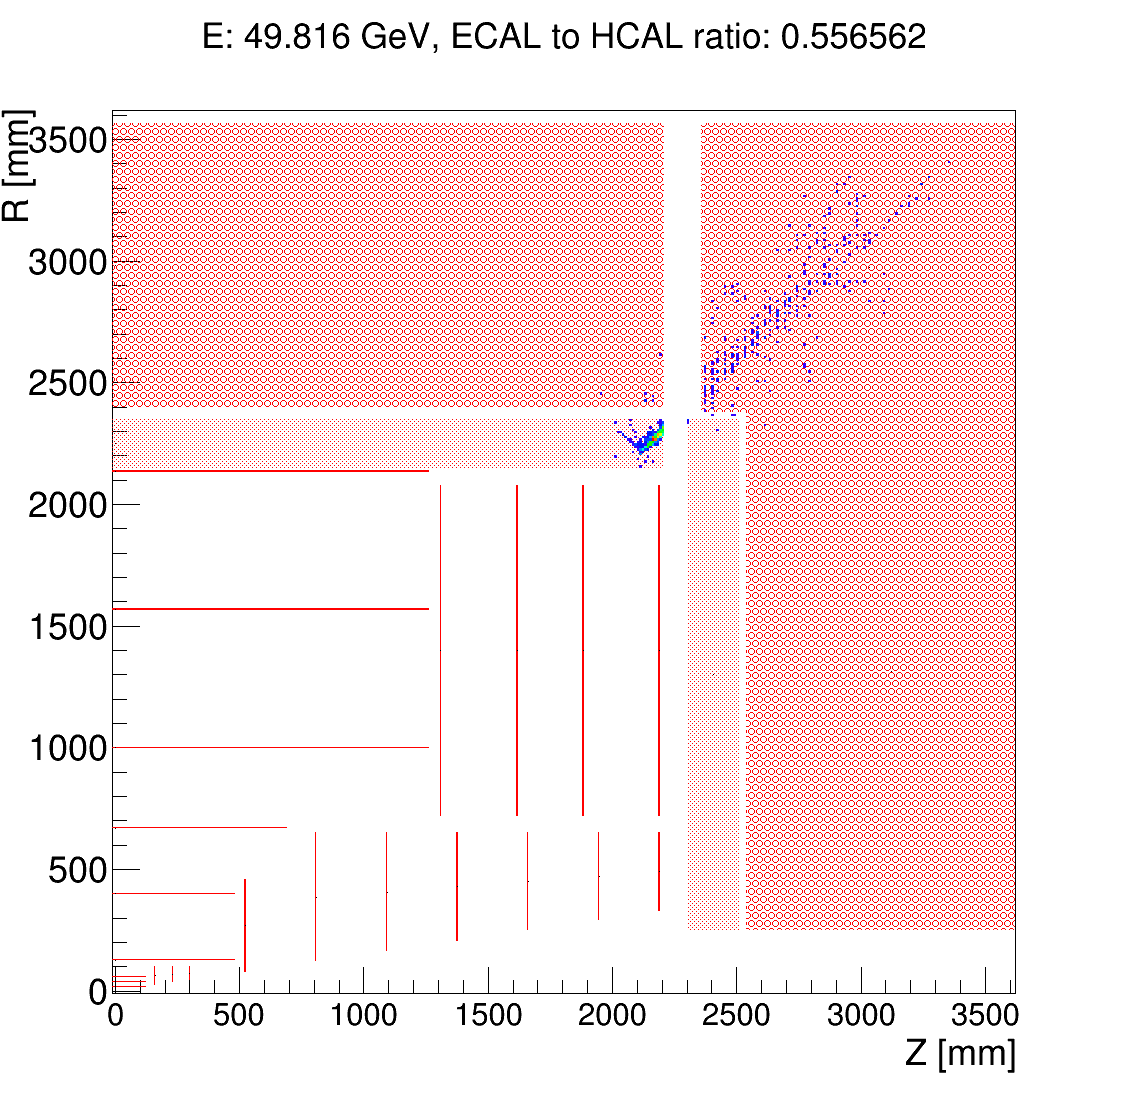
\includegraphics[width=5cm]{exHad2.png}};
  
  \node [Box] at (\xRefPosOne-1.4,\yRefPosOne) (box){%
    \myCenterBox{Photon PFOs}
  }; 

    \node [Box] at (\xRefPosOne+4.5,\yRefPosOne) (box){%
    \myCenterBox{Neutral PFOs}
  }; 
  

  
\end{tikzpicture}
\end{frame}
%*****************************************************************************

%*****************************************************************************
\begin{frame}{}
  \begin{tikzpicture}[overlay]
    \node[right] (textNode) at (1,0) {
      { \large \bf Electron and Pion ID efficiency in the transition region }
    };
  \end{tikzpicture}
\end{frame}
%*****************************************************************************

%*****************************************************************************
\begin{frame}{\large \large Electron and Pion ID efficiency in the transition region}
\renewcommand{\yRefPosOne}{-0.5}
\renewcommand{\xRefPosOne}{4.2}
\renewcommand{\xRefIncrementOne}{7.5}
\begin{tikzpicture}[overlay]

 \node[inner sep=0pt] (tmp) at (\xRefPosOne+4.6,\yRefPosOne+2)
  {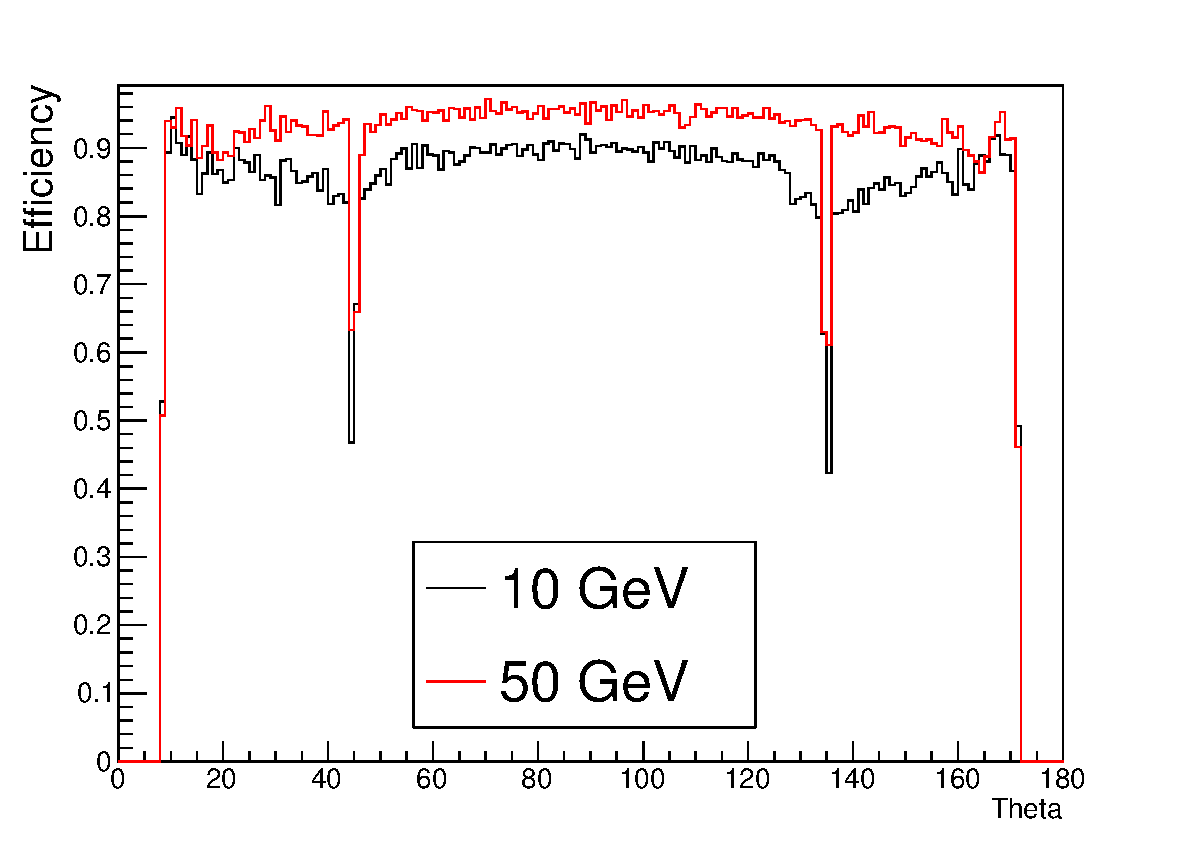
\includegraphics[width=6cm]{../Sep27_2017/thetaEff_e-.pdf}};
  
 \node[inner sep=0pt] (tmp) at (\xRefPosOne+4.6,\yRefPosOne-2.2)
  {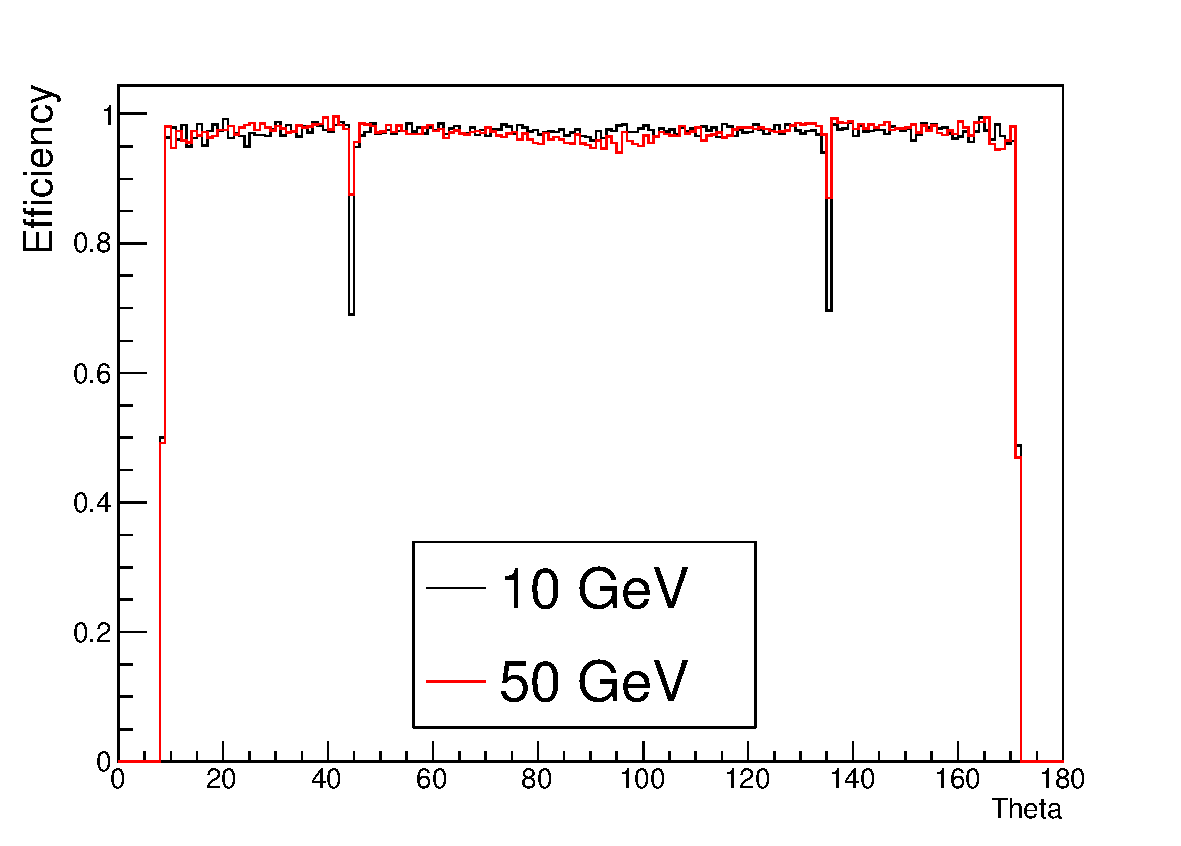
\includegraphics[width=6cm]{../Sep27_2017/thetaEff_pi-.pdf}};

\node [Box] at (\xRefPosOne+4.6,\yRefPosOne+-0.25) (box){%
  \myCenterBox{$\pi$-}
}; 

\node [Box] at (\xRefPosOne+4.6,\yRefPosOne+3.7) (box){%
\myCenterBox{$e$-}
}; 
  
\node[inner sep=0pt] (tmp) at (\xRefPosOne-1.7,\yRefPosOne+0.8)
  {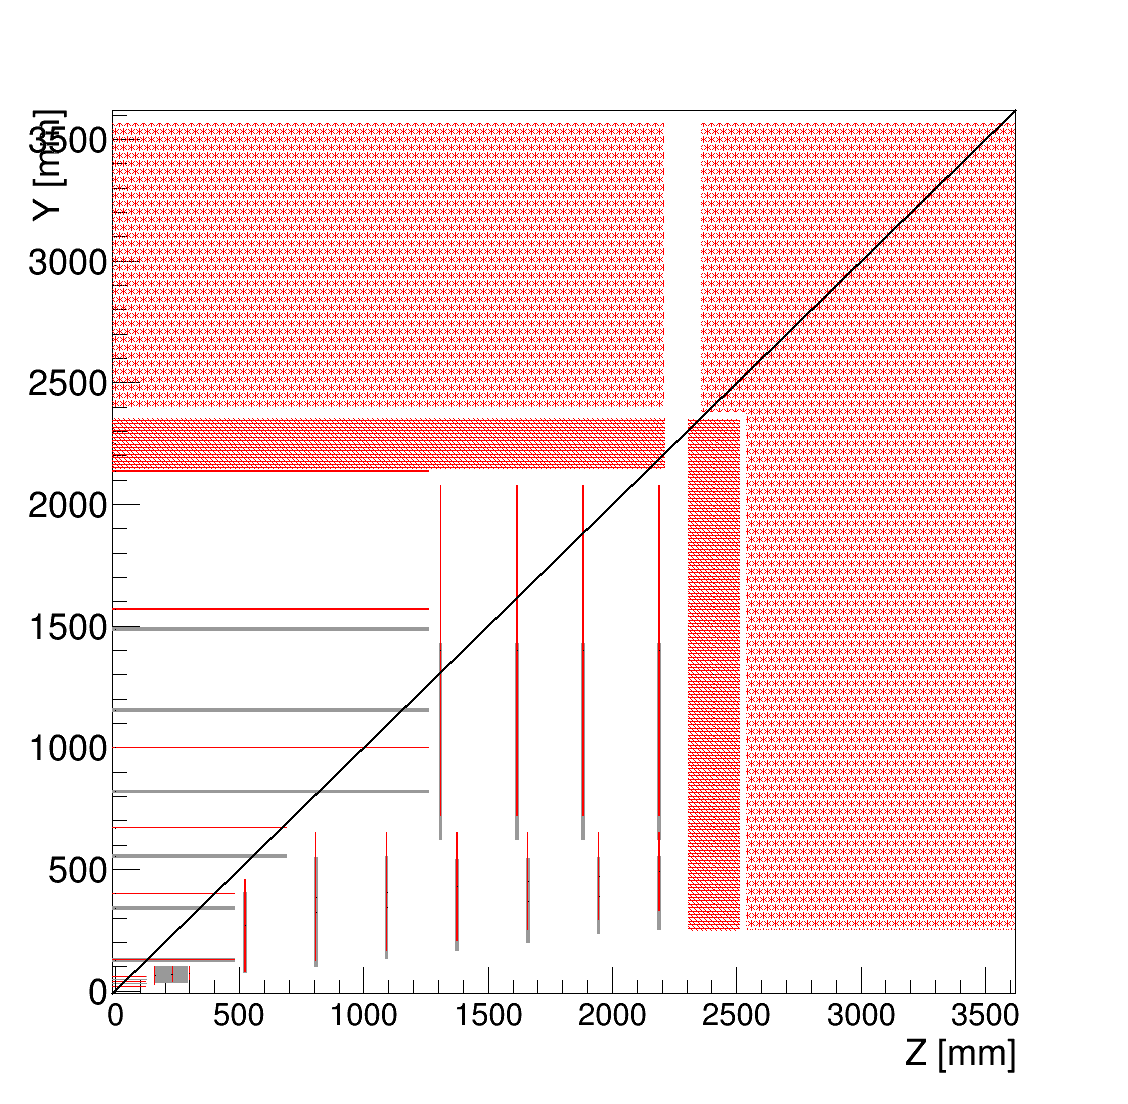
\includegraphics[width=6.7cm]{detectorGeometry.png}};
  

  
  \node [Box] at (\xRefPosOne-1.7,\yRefPosOne-3.2) (box){%
    \begin{minipage}{0.6\textwidth}
      \begin{itemize}
	\item Sofware issue with track-cluster association in the transition region
	\item Fixed in the latest iLCSoft release (to be confirmed)
      \end{itemize}
    \end{minipage}
  };
  
\end{tikzpicture}
\end{frame}
%*****************************************************************************

%*****************************************************************************
\begin{frame}{}
  \begin{tikzpicture}[overlay]
    \node[right] (textNode) at (2.4,0) {
      { \large \bf First look: jet energy resolution }
    };
  \end{tikzpicture}
\end{frame}
%*****************************************************************************

%*****************************************************************************
\begin{frame}{\large \large First look: jet energy resolution}
\renewcommand{\yRefPosOne}{-0.5}
\renewcommand{\xRefPosOne}{4.2}
\renewcommand{\xRefIncrementOne}{7.5}
\begin{tikzpicture}[overlay]

 \node[inner sep=0pt] (tmp) at (\xRefPosOne-1.7,\yRefPosOne+0.7)
  {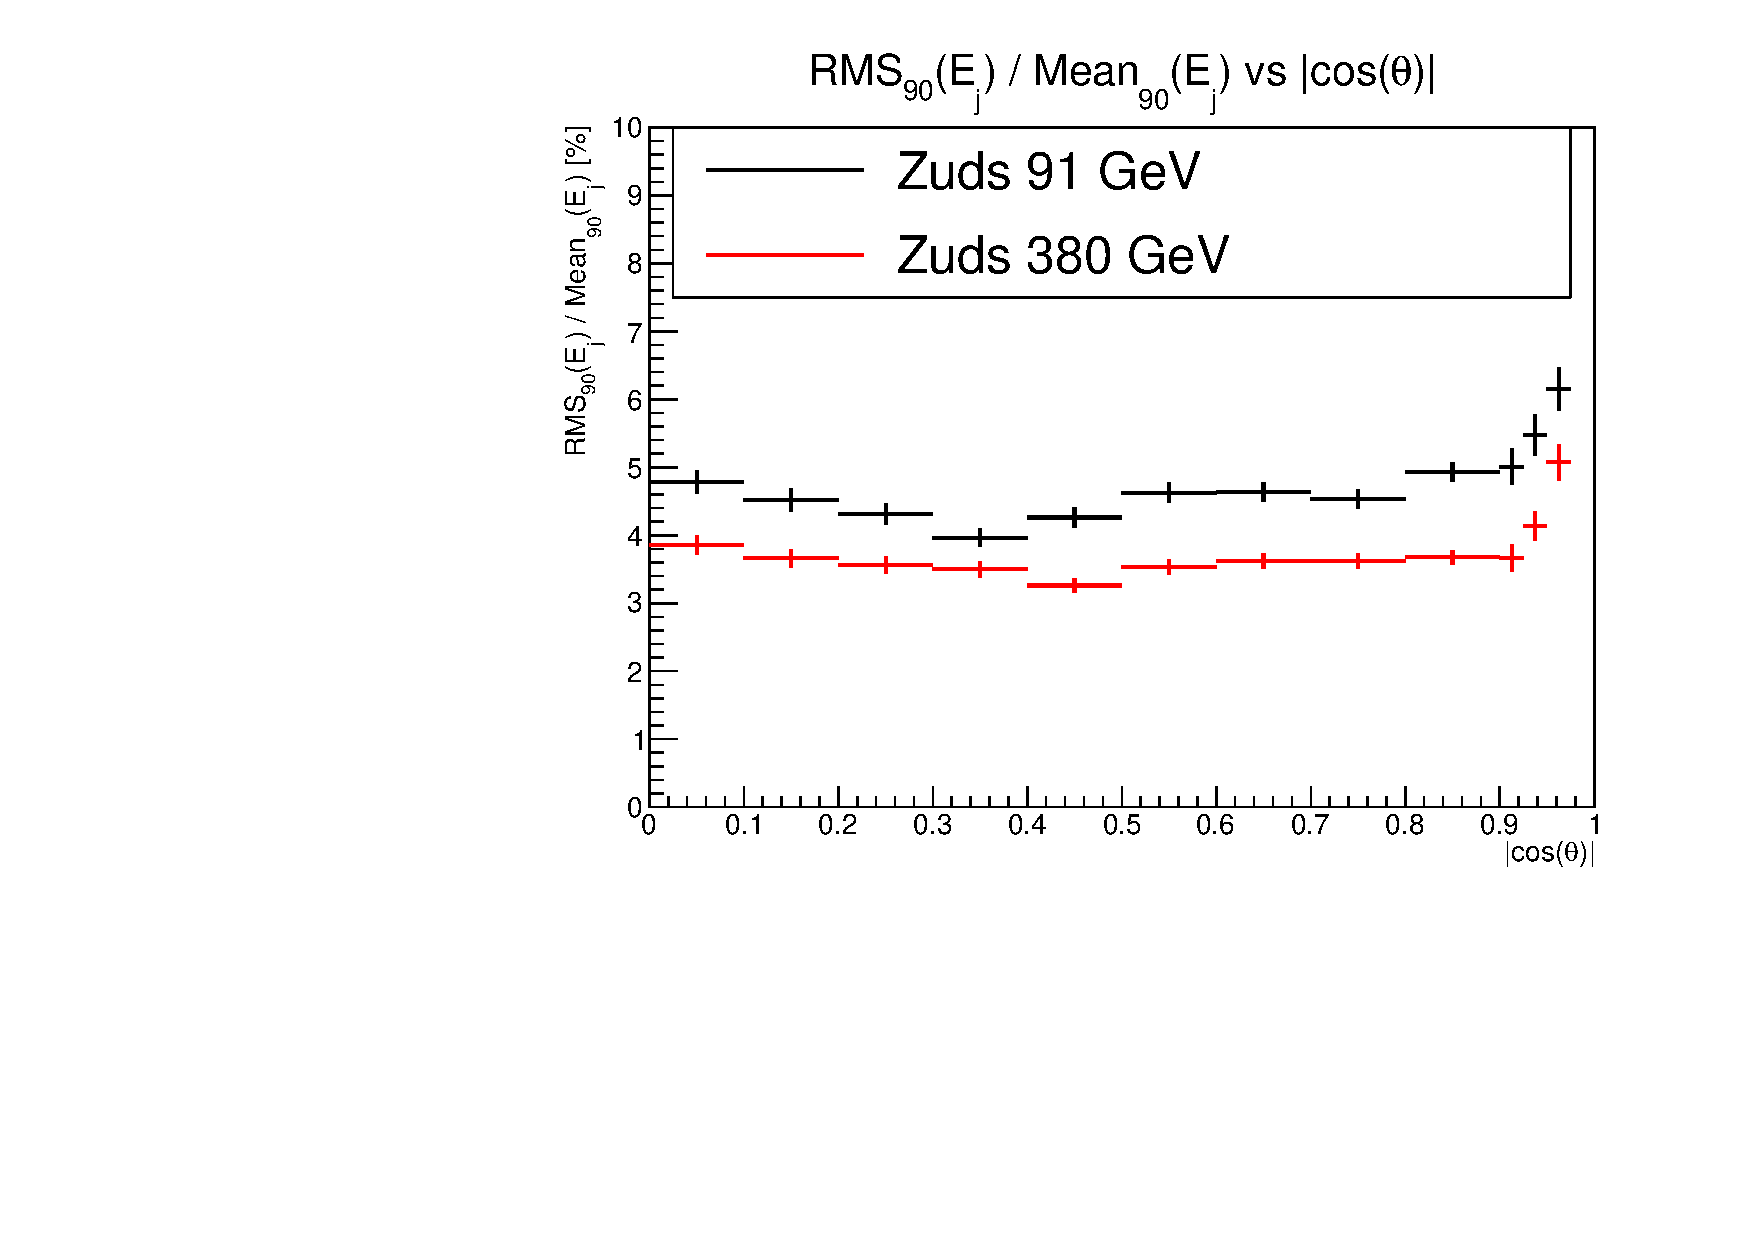
\includegraphics[width=6cm]{jet_energy_res.pdf}};
  
 \node[inner sep=0pt] (tmp) at (\xRefPosOne+4.5,\yRefPosOne+0.7)
  {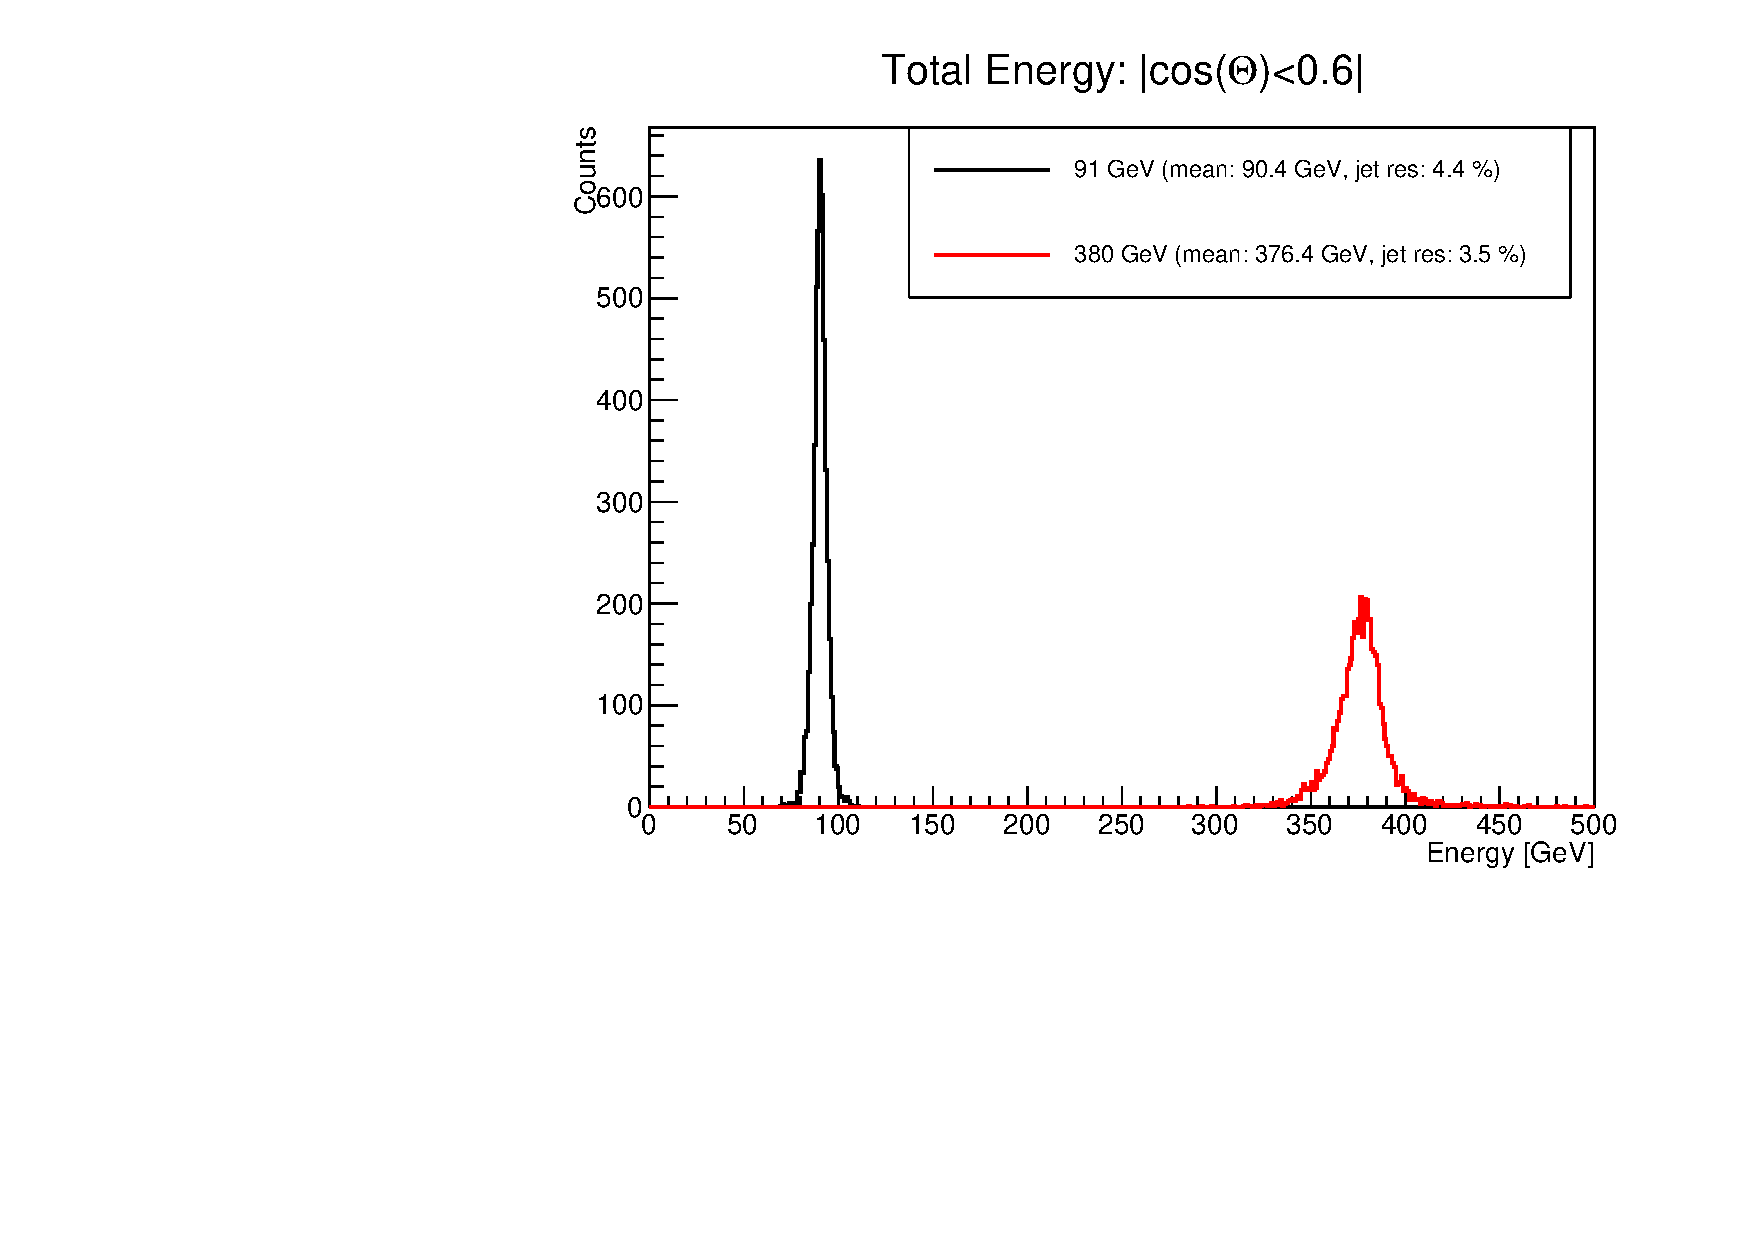
\includegraphics[width=6cm]{jet_energy.pdf}};

 \node[inner sep=0pt] (tmp) at (\xRefPosOne+4.5,\yRefPosOne-3)
  {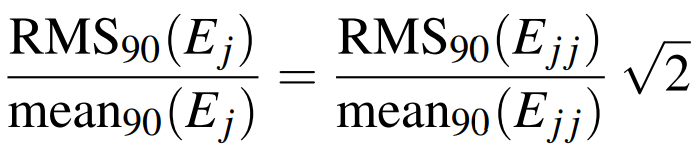
\includegraphics[width=4cm]{jetRes_formula.png}
  };
 
  \node[inner sep=0pt] (tmp) at (\xRefPosOne+4.5,\yRefPosOne-3.7)
  {\myCenterBox[yellow]{\href{http://arxiv.org/abs/1209.4039}{arXiv:1209.4039}}  };
 
 
 
 
 
  \node [Box] at (\xRefPosOne-0.3,\yRefPosOne-3) (box){%
    \begin{minipage}{0.8\textwidth}
      \begin{itemize}
	\item Total energy is reconstructed with 1$\%$ accuracy:
	\begin{itemize}
	 \item 91 GeV: \hspace{0.07cm} 90.4 GeV
	 \item 380 GeV: 376.4 GeV
	\end{itemize}
	\item Jet energy resolution in barrel region:
	\begin{itemize}
	 \item 91 GeV: \hspace{0.07cm} 3.5 $\%$
	 \item 380 GeV: 4.4 $\%$
	\end{itemize}

      \end{itemize}
    \end{minipage}
  };
  
\end{tikzpicture}
\end{frame}
%*****************************************************************************

%*****************************************************************************
\begin{frame}{}
  \begin{tikzpicture}[overlay]
    \node[right] (textNode) at (4.0,0) {
      { \large \bf Summary }
    };
  \end{tikzpicture}
\end{frame}
%*****************************************************************************

%*****************************************************************************
\begin{frame}{\large \large Summary}
 
\renewcommand{\yRefPosOne}{0.4}
\renewcommand{\xRefPosOne}{2.5}
\renewcommand{\xRefIncrementOne}{5.5}
\begin{tikzpicture}[overlay]

\node [Box] at (\xRefPosOne+2.5,\yRefPosOne+1) (box){%
  \begin{minipage}{\textwidth}
    \begin{itemize}
      \item Single particle ID performance with Pandora is understood\\ \vspace{0.2cm}
      \item Definition of the signle ID efficiency to use for CDR:
      \begin{itemize}
       \item angular matching (as used in the CLIC CDR)
       \item energy matching\\ \vspace{0.1cm}
      \end{itemize}
      \item Study on the jet energy reconstruction performance is started\\ \vspace{0.2cm}
    \end{itemize}
  \end{minipage}
};

\node [Box] at (\xRefPosOne+2.5,\yRefPosOne-2) (box){%
  \begin{minipage}{\textwidth}
    \begin{itemize}
      \item FCCee detector model is commited to the official iLCSoft repository
      \begin{itemize}
       \item current det. version: FCCee$\_$o1$\_$v01
      \end{itemize}
      \item Allows central production of the samples $\to$ detector performance with background overlaid
    \end{itemize}
  \end{minipage}
};
    

\end{tikzpicture}

  
\end{frame}
%*****************************************************************************

\end{document}

